%%%%%%%%%%%%%%%%%%%%%%%%%%%%%%%%%%%%%%%%%
% The Legrand Orange Book
% LaTeX Template
% Version 2.4 (26/09/2018)
%
% This template was downloaded from:
% http://www.LaTeXTemplates.com
%
% Original author:
% Mathias Legrand (legrand.mathias@gmail.com) with modifications by:
% Vel (vel@latextemplates.com)
%
% License:
% CC BY-NC-SA 3.0 (http://creativecommons.org/licenses/by-nc-sa/3.0/)
%
% Compiling this template:
% This template uses biber for its bibliography and makeindex for its index.
% When you first open the template, compile it from the command line with the 
% commands below to make sure your LaTeX distribution is configured correctly:
%
% 1) pdflatex main
% 2) makeindex main.idx -s StyleInd.ist
% 3) biber main
% 4) pdflatex main x 2
%
% After this, when you wish to update the bibliography/index use the appropriate
% command above and make sure to compile with pdflatex several times 
% afterwards to propagate your changes to the document.
%
% This template also uses a number of packages which may need to be
% updated to the newest versions for the template to compile. It is strongly
% recommended you update your LaTeX distribution if you have any
% compilation errors.
%
% Important note:
% Chapter heading images should have a 2:1 width:height ratio,
% e.g. 920px width and 460px height.
%
%%%%%%%%%%%%%%%%%%%%%%%%%%%%%%%%%%%%%%%%%

%----------------------------------------------------------------------------------------
%	PACKAGES AND OTHER DOCUMENT CONFIGURATIONS
%----------------------------------------------------------------------------------------
\documentclass[11pt,fleqn]{book} % Default font size and left-justified equations

%%%%%%%%%%%%%%%%%%%%%%%%%%%%%%%%%%%%%%%%%
% The Legrand Orange Book
% Structural Definitions File
% Version 2.1 (26/09/2018)
%
% Original author:
% Mathias Legrand (legrand.mathias@gmail.com) with modifications by:
% Vel (vel@latextemplates.com)
% 
% This file was downloaded from:
% http://www.LaTeXTemplates.com
%
% License:
% CC BY-NC-SA 3.0 (http://creativecommons.org/licenses/by-nc-sa/3.0/)
%
%%%%%%%%%%%%%%%%%%%%%%%%%%%%%%%%%%%%%%%%%

%----------------------------------------------------------------------------------------
%	VARIOUS REQUIRED PACKAGES AND CONFIGURATIONS
%----------------------------------------------------------------------------------------

\usepackage{graphicx} % Required for including pictures
\graphicspath{{Pictures/}} % Specifies the directory where pictures are stored

\usepackage{lipsum} % Inserts dummy text

\usepackage{tikz} % Required for drawing custom shapes

\usepackage[english]{babel} % English language/hyphenation

\usepackage{enumitem} % Customize lists
\setlist{nolistsep} % Reduce spacing between bullet points and numbered lists

\usepackage{booktabs} % Required for nicer horizontal rules in tables

\usepackage{xcolor} % Required for specifying colors by name
\definecolor{ocre}{RGB}{38, 100, 168} % Define the bluecolor used for highlighting throughout the book

%----------------------------------------------------------------------------------------
%	MARGINS
%----------------------------------------------------------------------------------------

\usepackage{geometry} % Required for adjusting page dimensions and margins

\geometry{
	paper=a4paper, % Paper size, change to letterpaper for US letter size
	top=3cm, % Top margin
	bottom=3cm, % Bottom margin
	left=3cm, % Left margin
	right=3cm, % Right margin
	headheight=14pt, % Header height
	footskip=1.4cm, % Space from the bottom margin to the baseline of the footer
	headsep=10pt, % Space from the top margin to the baseline of the header
	%showframe, % Uncomment to show how the type block is set on the page
}

%----------------------------------------------------------------------------------------
%	FONTS
%----------------------------------------------------------------------------------------

\usepackage{avant} % Use the Avantgarde font for headings
%\usepackage{times} % Use the Times font for headings
\usepackage{mathptmx} % Use the Adobe Times Roman as the default text font together with math symbols from the Sym­bol, Chancery and Com­puter Modern fonts

\usepackage{microtype} % Slightly tweak font spacing for aesthetics
\usepackage[utf8]{inputenc} % Required for including letters with accents
\usepackage[T1]{fontenc} % Use 8-bit encoding that has 256 glyphs

%----------------------------------------------------------------------------------------
%	BIBLIOGRAPHY AND INDEX
%----------------------------------------------------------------------------------------

\usepackage[style=numeric,citestyle=numeric,sorting=nyt,sortcites=true,autopunct=true,hyperref=true,abbreviate=false,backref=true,backend=biber]{biblatex}
\addbibresource{bibliography.bib} % BibTeX bibliography file
\defbibheading{bibempty}{}

\usepackage{calc} % For simpler calculation - used for spacing the index letter headings correctly
\usepackage{makeidx} % Required to make an index
\makeindex % Tells LaTeX to create the files required for indexing

%----------------------------------------------------------------------------------------
%	MAIN TABLE OF CONTENTS
%----------------------------------------------------------------------------------------

\usepackage{titletoc} % Required for manipulating the table of contents

\contentsmargin{0cm} % Removes the default margin

% Part text styling (this is mostly taken care of in the PART HEADINGS section of this file)
\titlecontents{part}
	[0cm] % Left indentation
	{\addvspace{20pt}\bfseries} % Spacing and font options for parts
	{}
	{}
	{}

% Chapter text styling
\titlecontents{chapter}
	[1.25cm] % Left indentation
	{\addvspace{12pt}\large\sffamily\bfseries} % Spacing and font options for chapters
	{\color{ocre!60}\contentslabel[\Large\thecontentslabel]{1.25cm}\color{ocre}} % Formatting of numbered sections of this type
	{\color{ocre}} % Formatting of numberless sections of this type
	{\color{ocre!60}\normalsize\;\titlerule*[.5pc]{.}\;\thecontentspage} % Formatting of the filler to the right of the heading and the page number

% Section text styling
\titlecontents{section}
	[1.25cm] % Left indentation
	{\addvspace{3pt}\sffamily\bfseries} % Spacing and font options for sections
	{\contentslabel[\thecontentslabel]{1.25cm}} % Formatting of numbered sections of this type
	{} % Formatting of numberless sections of this type
	{\hfill\color{black}\thecontentspage} % Formatting of the filler to the right of the heading and the page number

% Subsection text styling
\titlecontents{subsection}
	[1.25cm] % Left indentation
	{\addvspace{1pt}\sffamily\small} % Spacing and font options for subsections
	{\contentslabel[\thecontentslabel]{1.25cm}} % Formatting of numbered sections of this type
	{} % Formatting of numberless sections of this type
	{\ \titlerule*[.5pc]{.}\;\thecontentspage} % Formatting of the filler to the right of the heading and the page number

% Figure text styling
\titlecontents{figure}
	[1.25cm] % Left indentation
	{\addvspace{1pt}\sffamily\small} % Spacing and font options for figures
	{\thecontentslabel\hspace*{1em}} % Formatting of numbered sections of this type
	{} % Formatting of numberless sections of this type
	{\ \titlerule*[.5pc]{.}\;\thecontentspage} % Formatting of the filler to the right of the heading and the page number

% Table text styling
\titlecontents{table}
	[1.25cm] % Left indentation
	{\addvspace{1pt}\sffamily\small} % Spacing and font options for tables
	{\thecontentslabel\hspace*{1em}} % Formatting of numbered sections of this type
	{} % Formatting of numberless sections of this type
	{\ \titlerule*[.5pc]{.}\;\thecontentspage} % Formatting of the filler to the right of the heading and the page number

%----------------------------------------------------------------------------------------
%	MINI TABLE OF CONTENTS IN PART HEADS
%----------------------------------------------------------------------------------------

% Chapter text styling
\titlecontents{lchapter}
	[0em] % Left indentation
	{\addvspace{15pt}\large\sffamily\bfseries} % Spacing and font options for chapters
	{\color{ocre}\contentslabel[\Large\thecontentslabel]{1.25cm}\color{ocre}} % Chapter number
	{}  
	{\color{ocre}\normalsize\sffamily\bfseries\;\titlerule*[.5pc]{.}\;\thecontentspage} % Page number

% Section text styling
\titlecontents{lsection}
	[0em] % Left indentation
	{\sffamily\small} % Spacing and font options for sections
	{\contentslabel[\thecontentslabel]{1.25cm}} % Section number
	{}
	{}

% Subsection text styling (note these aren't shown by default, display them by searchings this file for tocdepth and reading the commented text)
\titlecontents{lsubsection}
	[.5em] % Left indentation
	{\sffamily\footnotesize} % Spacing and font options for subsections
	{\contentslabel[\thecontentslabel]{1.25cm}}
	{}
	{}

%----------------------------------------------------------------------------------------
%	HEADERS AND FOOTERS
%----------------------------------------------------------------------------------------

\usepackage{fancyhdr} % Required for header and footer configuration

\pagestyle{fancy} % Enable the custom headers and footers

\renewcommand{\chaptermark}[1]{\markboth{\sffamily\normalsize\bfseries\chaptername\ \thechapter.\ #1}{}} % Styling for the current chapter in the header
\renewcommand{\sectionmark}[1]{\markright{\sffamily\normalsize\thesection\hspace{5pt}#1}{}} % Styling for the current section in the header

\fancyhf{} % Clear default headers and footers
\fancyhead[LE,RO]{\sffamily\normalsize\thepage} % Styling for the page number in the header
\fancyhead[LO]{\rightmark} % Print the nearest section name on the left side of odd pages
\fancyhead[RE]{\leftmark} % Print the current chapter name on the right side of even pages
%\fancyfoot[C]{\thepage} % Uncomment to include a footer

\renewcommand{\headrulewidth}{0.5pt} % Thickness of the rule under the header

\fancypagestyle{plain}{% Style for when a plain pagestyle is specified
	\fancyhead{}\renewcommand{\headrulewidth}{0pt}%
}

% Removes the header from odd empty pages at the end of chapters
\makeatletter
\renewcommand{\cleardoublepage}{
\clearpage\ifodd\c@page\else
\hbox{}
\vspace*{\fill}
\thispagestyle{empty}
\newpage
\fi}

%----------------------------------------------------------------------------------------
%	THEOREM STYLES
%----------------------------------------------------------------------------------------

\usepackage{amsmath,amsfonts,amssymb,amsthm} % For math equations, theorems, symbols, etc

\newcommand{\intoo}[2]{\mathopen{]}#1\,;#2\mathclose{[}}
\newcommand{\ud}{\mathop{\mathrm{{}d}}\mathopen{}}
\newcommand{\intff}[2]{\mathopen{[}#1\,;#2\mathclose{]}}
\renewcommand{\qedsymbol}{$\blacksquare$}
\newtheorem{notation}{Notitie}[chapter]

% Boxed/framed environments
\newtheoremstyle{ocrenumbox}% Theorem style name
{0pt}% Space above
{0pt}% Space below
{\normalfont}% Body font
{}% Indent amount
{\small\bf\sffamily\color{ocre}}% Theorem head font
{\;}% Punctuation after theorem head
{0.25em}% Space after theorem head
{\small\sffamily\color{ocre}\thmname{#1}\nobreakspace\thmnumber{\@ifnotempty{#1}{}\@upn{#2}}% Theorem text (e.g. Theorem 2.1)
\thmnote{\nobreakspace\the\thm@notefont\sffamily\bfseries\color{black}---\nobreakspace#3.}} % Optional theorem note

\newtheoremstyle{blacknumex}% Theorem style name
{5pt}% Space above
{5pt}% Space below
{\normalfont}% Body font
{} % Indent amount
{\small\bf\sffamily}% Theorem head font
{\;}% Punctuation after theorem head
{0.25em}% Space after theorem head
{\small\sffamily{\tiny\ensuremath{\blacksquare}}\nobreakspace\thmname{#1}\nobreakspace\thmnumber{\@ifnotempty{#1}{}\@upn{#2}}% Theorem text (e.g. Theorem 2.1)
\thmnote{\nobreakspace\the\thm@notefont\sffamily\bfseries---\nobreakspace#3.}}% Optional theorem note

\newtheoremstyle{blacknumbox} % Theorem style name
{0pt}% Space above
{0pt}% Space below
{\normalfont}% Body font
{}% Indent amount
{\small\bf\sffamily}% Theorem head font
{\;}% Punctuation after theorem head
{0.25em}% Space after theorem head
{\small\sffamily\thmname{#1}\nobreakspace\thmnumber{\@ifnotempty{#1}{}\@upn{#2}}% Theorem text (e.g. Theorem 2.1)
\thmnote{\nobreakspace\the\thm@notefont\sffamily\bfseries---\nobreakspace#3.}}% Optional theorem note

% Non-boxed/non-framed environments
\newtheoremstyle{ocrenum}% Theorem style name
{5pt}% Space above
{5pt}% Space below
{\normalfont}% Body font
{}% Indent amount
{\small\bf\sffamily\color{ocre}}% Theorem head font
{\;}% Punctuation after theorem head
{0.25em}% Space after theorem head
{\small\sffamily\color{ocre}\thmname{#1}\nobreakspace\thmnumber{\@ifnotempty{#1}{}\@upn{#2}}% Theorem text (e.g. Theorem 2.1)
\thmnote{\nobreakspace\the\thm@notefont\sffamily\bfseries\color{black}---\nobreakspace#3.}} % Optional theorem note
\makeatother

% Defines the theorem text style for each type of theorem to one of the three styles above
\newcounter{dummy} 
\numberwithin{dummy}{section}
\theoremstyle{ocrenumbox}
\newtheorem{theoremeT}[dummy]{Theorema}
\newtheorem{problem}{Probleem}[chapter]
\newtheorem{exerciseT}{Opdracht}[chapter]
\theoremstyle{blacknumex}
\newtheorem{exampleT}{Voorbeeld}[chapter]
\theoremstyle{blacknumbox}
\newtheorem{vocabulary}{Vocabulair}[chapter]
\newtheorem{definitionT}{Definitie}[section]
\newtheorem{corollaryT}[dummy]{Corollary}
\theoremstyle{ocrenum}
\newtheorem{proposition}[dummy]{Propositie}

%----------------------------------------------------------------------------------------
%	DEFINITION OF COLORED BOXES
%----------------------------------------------------------------------------------------

\RequirePackage[framemethod=default]{mdframed} % Required for creating the theorem, definition, exercise and corollary boxes

% Theorem box
\newmdenv[skipabove=7pt,
skipbelow=7pt,
backgroundcolor=black!5,
linecolor=ocre,
innerleftmargin=5pt,
innerrightmargin=5pt,
innertopmargin=5pt,
leftmargin=0cm,
rightmargin=0cm,
innerbottommargin=5pt]{tBox}

% Exercise box	  
\newmdenv[skipabove=7pt,
skipbelow=7pt,
rightline=false,
leftline=true,
topline=false,
bottomline=false,
backgroundcolor=ocre!10,
linecolor=ocre,
innerleftmargin=5pt,
innerrightmargin=5pt,
innertopmargin=5pt,
innerbottommargin=5pt,
leftmargin=0cm,
rightmargin=0cm,
linewidth=4pt]{eBox}	

% Definition box
\newmdenv[skipabove=7pt,
skipbelow=7pt,
rightline=false,
leftline=true,
topline=false,
bottomline=false,
linecolor=ocre,
innerleftmargin=5pt,
innerrightmargin=5pt,
innertopmargin=0pt,
leftmargin=0cm,
rightmargin=0cm,
linewidth=4pt,
innerbottommargin=0pt]{dBox}	

% Corollary box
\newmdenv[skipabove=7pt,
skipbelow=7pt,
rightline=false,
leftline=true,
topline=false,
bottomline=false,
linecolor=gray,
backgroundcolor=black!5,
innerleftmargin=5pt,
innerrightmargin=5pt,
innertopmargin=5pt,
leftmargin=0cm,
rightmargin=0cm,
linewidth=4pt,
innerbottommargin=5pt]{cBox}

% Creates an environment for each type of theorem and assigns it a theorem text style from the "Theorem Styles" section above and a colored box from above
\newenvironment{theorem}{\begin{tBox}\begin{theoremeT}}{\end{theoremeT}\end{tBox}}
\newenvironment{exercise}{\begin{eBox}\begin{exerciseT}}{\hfill{\color{ocre}\tiny\ensuremath{\blacksquare}}\end{exerciseT}\end{eBox}}				  
\newenvironment{definition}{\begin{dBox}\begin{definitionT}}{\end{definitionT}\end{dBox}}	
\newenvironment{example}{\begin{exampleT}}{\hfill{\tiny\ensuremath{\blacksquare}}\end{exampleT}}		
\newenvironment{corollary}{\begin{cBox}\begin{corollaryT}}{\end{corollaryT}\end{cBox}}	

%----------------------------------------------------------------------------------------
%	REMARK ENVIRONMENT
%----------------------------------------------------------------------------------------

\newenvironment{remark}{\par\vspace{10pt}\small % Vertical white space above the remark and smaller font size
\begin{list}{}{
\leftmargin=35pt % Indentation on the left
\rightmargin=25pt}\item\ignorespaces % Indentation on the right
\makebox[-2.5pt]{\begin{tikzpicture}[overlay]
\node[draw=ocre!60,line width=1pt,circle,fill=ocre!25,font=\sffamily\bfseries,inner sep=2pt,outer sep=0pt] at (-15pt,0pt){\textcolor{ocre}{N.B.}};\end{tikzpicture}} % Orange R in a circle
\advance\baselineskip -1pt}{\end{list}\vskip5pt} % Tighter line spacing and white space after remark

%----------------------------------------------------------------------------------------
%	SECTION NUMBERING IN THE MARGIN
%----------------------------------------------------------------------------------------

\makeatletter
\renewcommand{\@seccntformat}[1]{\llap{\textcolor{ocre}{\csname the#1\endcsname}\hspace{1em}}}                    
\renewcommand{\section}{\@startsection{section}{1}{\z@}
{-4ex \@plus -1ex \@minus -.4ex}
{1ex \@plus.2ex }
{\normalfont\large\sffamily\bfseries}}
\renewcommand{\subsection}{\@startsection {subsection}{2}{\z@}
{-3ex \@plus -0.1ex \@minus -.4ex}
{0.5ex \@plus.2ex }
{\normalfont\sffamily\bfseries}}
\renewcommand{\subsubsection}{\@startsection {subsubsection}{3}{\z@}
{-2ex \@plus -0.1ex \@minus -.2ex}
{.2ex \@plus.2ex }
{\normalfont\small\sffamily\bfseries}}                        
\renewcommand\paragraph{\@startsection{paragraph}{4}{\z@}
{-2ex \@plus-.2ex \@minus .2ex}
{.1ex}
{\normalfont\small\sffamily\bfseries}}

%----------------------------------------------------------------------------------------
%	PART HEADINGS
%----------------------------------------------------------------------------------------

% Numbered part in the table of contents
\newcommand{\@mypartnumtocformat}[2]{%
	\setlength\fboxsep{0pt}%
	\noindent\colorbox{ocre!20}{\strut\parbox[c][.7cm]{\ecart}{\color{ocre!70}\Large\sffamily\bfseries\centering#1}}\hskip\esp\colorbox{ocre!40}{\strut\parbox[c][.7cm]{\linewidth-\ecart-\esp}{\Large\sffamily\centering#2}}%
}

% Unnumbered part in the table of contents
\newcommand{\@myparttocformat}[1]{%
	\setlength\fboxsep{0pt}%
	\noindent\colorbox{ocre!40}{\strut\parbox[c][.7cm]{\linewidth}{\Large\sffamily\centering#1}}%
}

\newlength\esp
\setlength\esp{4pt}
\newlength\ecart
\setlength\ecart{1.2cm-\esp}
\newcommand{\thepartimage}{}%
\newcommand{\partimage}[1]{\renewcommand{\thepartimage}{#1}}%
\def\@part[#1]#2{%
\ifnum \c@secnumdepth >-2\relax%
\refstepcounter{part}%
\addcontentsline{toc}{part}{\texorpdfstring{\protect\@mypartnumtocformat{\thepart}{#1}}{\partname~\thepart\ ---\ #1}}
\else%
\addcontentsline{toc}{part}{\texorpdfstring{\protect\@myparttocformat{#1}}{#1}}%
\fi%
\startcontents%
\markboth{}{}%
{\thispagestyle{empty}%
\begin{tikzpicture}[remember picture,overlay]%
\node at (current page.north west){\begin{tikzpicture}[remember picture,overlay]%	
\fill[ocre!20](0cm,0cm) rectangle (\paperwidth,-\paperheight);
\node[anchor=north] at (4cm,-3.25cm){\color{ocre!40}\fontsize{220}{100}\sffamily\bfseries\thepart}; 
\node[anchor=south east] at (\paperwidth-1cm,-\paperheight+1cm){\parbox[t][][t]{8.5cm}{
\printcontents{l}{0}{\setcounter{tocdepth}{1}}% The depth to which the Part mini table of contents displays headings; 0 for chapters only, 1 for chapters and sections and 2 for chapters, sections and subsections
}};
\node[anchor=north east] at (\paperwidth-1.5cm,-3.25cm){\parbox[t][][t]{15cm}{\strut\raggedleft\color{white}\fontsize{30}{30}\sffamily\bfseries#2}};
\end{tikzpicture}};
\end{tikzpicture}}%
\@endpart}
\def\@spart#1{%
\startcontents%
\phantomsection
{\thispagestyle{empty}%
\begin{tikzpicture}[remember picture,overlay]%
\node at (current page.north west){\begin{tikzpicture}[remember picture,overlay]%	
\fill[ocre!20](0cm,0cm) rectangle (\paperwidth,-\paperheight);
\node[anchor=north east] at (\paperwidth-1.5cm,-3.25cm){\parbox[t][][t]{15cm}{\strut\raggedleft\color{white}\fontsize{30}{30}\sffamily\bfseries#1}};
\end{tikzpicture}};
\end{tikzpicture}}
\addcontentsline{toc}{part}{\texorpdfstring{%
\setlength\fboxsep{0pt}%
\noindent\protect\colorbox{ocre!40}{\strut\protect\parbox[c][.7cm]{\linewidth}{\Large\sffamily\protect\centering #1\quad\mbox{}}}}{#1}}%
\@endpart}
\def\@endpart{\vfil\newpage
\if@twoside
\if@openright
\null
\thispagestyle{empty}%
\newpage
\fi
\fi
\if@tempswa
\twocolumn
\fi}

%----------------------------------------------------------------------------------------
%	CHAPTER HEADINGS
%----------------------------------------------------------------------------------------
\setlength{\parindent}{0em}
% A switch to conditionally include a picture, implemented by Christian Hupfer
\newif\ifusechapterimage
\usechapterimagetrue
\newcommand{\thechapterimage}{}%
\newcommand{\chapterimage}[1]{\ifusechapterimage\renewcommand{\thechapterimage}{#1}\fi}%
\newcommand{\autodot}{.}
\def\@makechapterhead#1{%
{\parindent \z@ \raggedright \normalfont
\ifnum \c@secnumdepth >\m@ne
\if@mainmatter
\begin{tikzpicture}[remember picture,overlay]
\node at (current page.north west)
{\begin{tikzpicture}[remember picture,overlay]
\node[anchor=north west,inner sep=0pt] at (0,0) {\ifusechapterimage\includegraphics[width=\paperwidth]{\thechapterimage}\fi};
\draw[anchor=west] (\Gm@lmargin,-9cm) node [line width=2pt,rounded corners=15pt,draw=ocre,fill=white,fill opacity=0.5,inner sep=15pt]{\strut\makebox[22cm]{}};
\draw[anchor=west] (\Gm@lmargin+.3cm,-9cm) node {\huge\sffamily\bfseries\color{black}\thechapter\autodot~#1\strut};
\end{tikzpicture}};
\end{tikzpicture}
\else
\begin{tikzpicture}[remember picture,overlay]
\node at (current page.north west)
{\begin{tikzpicture}[remember picture,overlay]
\node[anchor=north west,inner sep=0pt] at (0,0) {\ifusechapterimage\includegraphics[width=\paperwidth]{\thechapterimage}\fi};
\draw[anchor=west] (\Gm@lmargin,-9cm) node [line width=2pt,rounded corners=15pt,draw=ocre,fill=white,fill opacity=0.5,inner sep=15pt]{\strut\makebox[22cm]{}};
\draw[anchor=west] (\Gm@lmargin+.3cm,-9cm) node {\huge\sffamily\bfseries\color{black}#1\strut};
\end{tikzpicture}};
\end{tikzpicture}
\fi\fi\par\vspace*{270\p@}}}

%-------------------------------------------

\def\@makeschapterhead#1{%
\begin{tikzpicture}[remember picture,overlay]
\node at (current page.north west)
{\begin{tikzpicture}[remember picture,overlay]
\node[anchor=north west,inner sep=0pt] at (0,0) {\ifusechapterimage\includegraphics[width=\paperwidth]{\thechapterimage}\fi};
\draw[anchor=west] (\Gm@lmargin,-9cm) node [line width=2pt,rounded corners=15pt,draw=ocre,fill=white,fill opacity=0.5,inner sep=15pt]{\strut\makebox[22cm]{}};
\draw[anchor=west] (\Gm@lmargin+.3cm,-9cm) node {\huge\sffamily\bfseries\color{black}#1\strut};
\end{tikzpicture}};
\end{tikzpicture}
\par\vspace*{270\p@}}
\makeatother

%----------------------------------------------------------------------------------------
%	LINKS
%----------------------------------------------------------------------------------------

\usepackage{hyperref}
\hypersetup{hidelinks,backref=true,pagebackref=true,hyperindex=true,colorlinks=false,breaklinks=true,urlcolor=ocre,bookmarks=true,bookmarksopen=false}

\usepackage{bookmark}
\bookmarksetup{
open,
numbered,
addtohook={%
\ifnum\bookmarkget{level}=0 % chapter
\bookmarksetup{bold}%
\fi
\ifnum\bookmarkget{level}=-1 % part
\bookmarksetup{color=ocre,bold}%
\fi
}
}

%----------------------------------------------------------------------------------------
% ACRONYMS	
%----------------------------------------------------------------------------------------
\usepackage{acronym}

%----------------------------------------------------------------------------------------
%	LISTINGS
%----------------------------------------------------------------------------------------
\usepackage{color}
\usepackage{listings}    
\usepackage{courier}

%%% Define Custom IDE Colors %%%
\definecolor{arduinoGreen}    {rgb} {0.17, 0.43, 0.01}
\definecolor{arduinoGrey}     {rgb} {0.47, 0.47, 0.33}
\definecolor{arduinoOrange}   {rgb} {0.8 , 0.4 , 0   }
\definecolor{arduinoBlue}     {rgb} {0.01, 0.61, 0.98}
\definecolor{arduinoDarkBlue} {rgb} {0.0 , 0.2 , 0.5 }

%%% Define Arduino Language %%%
\lstdefinelanguage{Arduino}{
  language=C++, % begin with default C++ settings 
%
%
  %%% Keyword Color Group 1 %%%  (called KEYWORD3 by arduino)
  keywordstyle=\color{arduinoGreen},   
  deletekeywords={  % remove all arduino keywords that might be in c++
                break, case, override, final, continue, default, do, else, for, 
                if, return, goto, switch, throw, try, while, setup, loop, export, 
                not, or, and, xor, include, define, elif, else, error, if, ifdef, 
                ifndef, pragma, warning,
                HIGH, LOW, INPUT, INPUT_PULLUP, OUTPUT, DEC, BIN, HEX, OCT, PI, 
                HALF_PI, TWO_PI, LSBFIRST, MSBFIRST, CHANGE, FALLING, RISING, 
                DEFAULT, EXTERNAL, INTERNAL, INTERNAL1V1, INTERNAL2V56, LED_BUILTIN, 
                LED_BUILTIN_RX, LED_BUILTIN_TX, DIGITAL_MESSAGE, FIRMATA_STRING, 
                ANALOG_MESSAGE, REPORT_DIGITAL, REPORT_ANALOG, SET_PIN_MODE, 
                SYSTEM_RESET, SYSEX_START, auto, int8_t, int16_t, int32_t, int64_t, 
                uint8_t, uint16_t, uint32_t, uint64_t, char16_t, char32_t, operator, 
                enum, delete, bool, boolean, byte, char, const, false, float, double, 
                null, NULL, int, long, new, private, protected, public, short, 
                signed, static, volatile, String, void, true, unsigned, word, array, 
                sizeof, dynamic_cast, typedef, const_cast, struct, static_cast, union, 
                friend, extern, class, reinterpret_cast, register, explicit, inline, 
                _Bool, complex, _Complex, _Imaginary, atomic_bool, atomic_char, 
                atomic_schar, atomic_uchar, atomic_short, atomic_ushort, atomic_int, 
                atomic_uint, atomic_long, atomic_ulong, atomic_llong, atomic_ullong, 
                virtual, PROGMEM,
                Serial, Serial1, Serial2, Serial3, SerialUSB, Keyboard, Mouse,
                abs, acos, asin, atan, atan2, ceil, constrain, cos, degrees, exp, 
                floor, log, map, max, min, radians, random, randomSeed, round, sin, 
                sq, sqrt, tan, pow, bitRead, bitWrite, bitSet, bitClear, bit, 
                highByte, lowByte, analogReference, analogRead, 
                analogReadResolution, analogWrite, analogWriteResolution, 
                attachInterrupt, detachInterrupt, digitalPinToInterrupt, delay, 
                delayMicroseconds, digitalWrite, digitalRead, interrupts, millis, 
                micros, noInterrupts, noTone, pinMode, pulseIn, pulseInLong, shiftIn, 
                shiftOut, tone, yield, Stream, begin, end, peek, read, print, 
                println, available, availableForWrite, flush, setTimeout, find, 
                findUntil, parseInt, parseFloat, readBytes, readBytesUntil, readString, 
                readStringUntil, trim, toUpperCase, toLowerCase, charAt, compareTo, 
                concat, endsWith, startsWith, equals, equalsIgnoreCase, getBytes, 
                indexOf, lastIndexOf, length, replace, setCharAt, substring, 
                toCharArray, toInt, press, release, releaseAll, accept, click, move, 
                isPressed, isAlphaNumeric, isAlpha, isAscii, isWhitespace, isControl, 
                isDigit, isGraph, isLowerCase, isPrintable, isPunct, isSpace, 
                isUpperCase, isHexadecimalDigit, 
                }, 
  morekeywords={   % add arduino structures to group 1
                break, case, override, final, continue, default, do, else, for, 
                if, return, goto, switch, throw, try, while, setup, loop, export, 
                not, or, and, xor, include, define, elif, else, error, if, ifdef, 
                ifndef, pragma, warning,
                }, 
% 
%
  %%% Keyword Color Group 2 %%%  (called LITERAL1 by arduino)
  keywordstyle=[2]\color{arduinoBlue},   
  keywords=[2]{   % add variables and dataTypes as 2nd group  
                HIGH, LOW, INPUT, INPUT_PULLUP, OUTPUT, DEC, BIN, HEX, OCT, PI, 
                HALF_PI, TWO_PI, LSBFIRST, MSBFIRST, CHANGE, FALLING, RISING, 
                DEFAULT, EXTERNAL, INTERNAL, INTERNAL1V1, INTERNAL2V56, LED_BUILTIN, 
                LED_BUILTIN_RX, LED_BUILTIN_TX, DIGITAL_MESSAGE, FIRMATA_STRING, 
                ANALOG_MESSAGE, REPORT_DIGITAL, REPORT_ANALOG, SET_PIN_MODE, 
                SYSTEM_RESET, SYSEX_START, auto, int8_t, int16_t, int32_t, int64_t, 
                uint8_t, uint16_t, uint32_t, uint64_t, char16_t, char32_t, operator, 
                enum, delete, bool, boolean, byte, char, const, false, float, double, 
                null, NULL, int, long, new, private, protected, public, short, 
                signed, static, volatile, String, void, true, unsigned, word, array, 
                sizeof, dynamic_cast, typedef, const_cast, struct, static_cast, union, 
                friend, extern, class, reinterpret_cast, register, explicit, inline, 
                _Bool, complex, _Complex, _Imaginary, atomic_bool, atomic_char, 
                atomic_schar, atomic_uchar, atomic_short, atomic_ushort, atomic_int, 
                atomic_uint, atomic_long, atomic_ulong, atomic_llong, atomic_ullong, 
                virtual, PROGMEM,
                },  
% 
%
  %%% Keyword Color Group 3 %%%  (called KEYWORD1 by arduino)
  keywordstyle=[3]\bfseries\color{arduinoOrange},
  keywords=[3]{  % add built-in functions as a 3rd group
                Serial, Serial1, Serial2, Serial3, SerialUSB, Keyboard, Mouse,
                },      
%
%
  %%% Keyword Color Group 4 %%%  (called KEYWORD2 by arduino)
  keywordstyle=[4]\color{arduinoOrange},
  keywords=[4]{  % add more built-in functions as a 4th group
                abs, acos, asin, atan, atan2, ceil, constrain, cos, degrees, exp, 
                floor, log, map, max, min, radians, random, randomSeed, round, sin, 
                sq, sqrt, tan, pow, bitRead, bitWrite, bitSet, bitClear, bit, 
                highByte, lowByte, analogReference, analogRead, 
                analogReadResolution, analogWrite, analogWriteResolution, 
                attachInterrupt, detachInterrupt, digitalPinToInterrupt, delay, 
                delayMicroseconds, digitalWrite, digitalRead, interrupts, millis, 
                micros, noInterrupts, noTone, pinMode, pulseIn, pulseInLong, shiftIn, 
                shiftOut, tone, yield, Stream, begin, end, peek, read, print, 
                println, available, availableForWrite, flush, setTimeout, find, 
                findUntil, parseInt, parseFloat, readBytes, readBytesUntil, readString, 
                readStringUntil, trim, toUpperCase, toLowerCase, charAt, compareTo, 
                concat, endsWith, startsWith, equals, equalsIgnoreCase, getBytes, 
                indexOf, lastIndexOf, length, replace, setCharAt, substring, 
                toCharArray, toInt, press, release, releaseAll, accept, click, move, 
                isPressed, isAlphaNumeric, isAlpha, isAscii, isWhitespace, isControl, 
                isDigit, isGraph, isLowerCase, isPrintable, isPunct, isSpace, 
                isUpperCase, isHexadecimalDigit, 
                },      
%
%
  %%% Set Other Colors %%%
  stringstyle=\color{arduinoDarkBlue},    
  commentstyle=\color{arduinoGrey},    
%          
%   
  %%%% Line Numbering %%%%
   numbers=left,                    
  numbersep=5pt,                   
  numberstyle=\color{arduinoGrey},    
  %stepnumber=2,                      % show every 2 line numbers
%
%
  %%%% Code Box Style %%%%
  breaklines=true,                    % wordwrapping
  tabsize=2,         
  frame=single,
  basicstyle=\ttfamily
}
 % Insert the commands.tex file which contains the majority of the structure behind the template

\hypersetup{pdftitle={Programmeren 2: Huiswerkopdrachten (Ad IA\&R)},pdfauthor={Stefan Rolink}} 

%----------------------------------------------------------------------------------------

\begin{document}

%----------------------------------------------------------------------------------------
%	TITLE PAGE
%----------------------------------------------------------------------------------------

\begingroup
\thispagestyle{empty} % Suppress headers and footers on the title page
\begin{tikzpicture}[remember picture,overlay]
\node[inner sep=0pt] (background) at (current page.center) {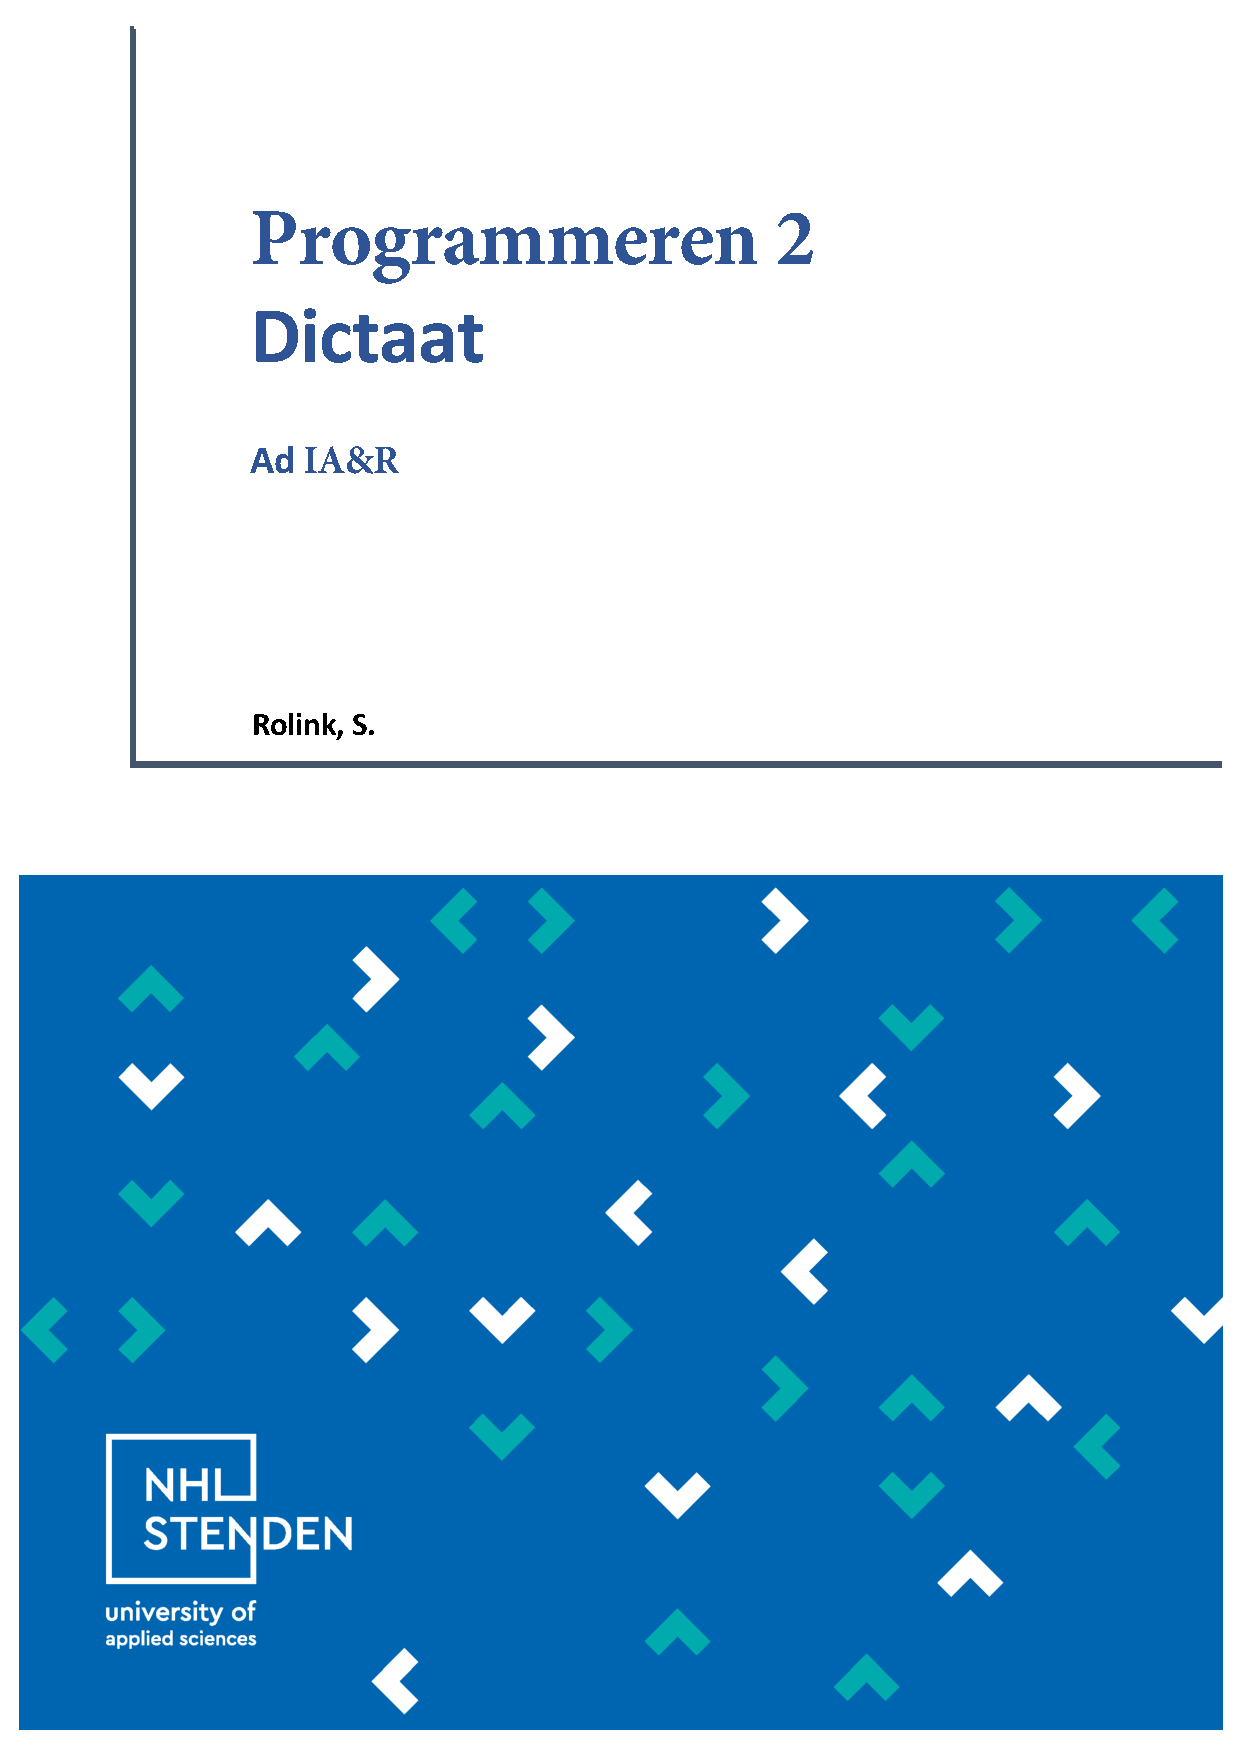
\includegraphics[width=\paperwidth]{NHL_cover_P2.pdf}};
% \draw (current page.center) node [fill=ocre!30!white,fill opacity=0,text opacity=1,inner sep=1cm]{\Huge\bfseries\sffamily\parbox[c][][t]{\paperwidth}{\\[15pt] % Book title
% {\huge }\\[20pt] % Subtitle
% {\Large }}}; % Author name
\end{tikzpicture}
\vfill
\endgroup

%----------------------------------------------------------------------------------------
%	COPYRIGHT PAGE
%----------------------------------------------------------------------------------------

\newpage
~\vfill
\thispagestyle{empty}

\noindent Copyright \copyright\ 2021 Stefan Rolink % Copyright notice

\noindent \textsc{Published by NHL Stenden} % Publisher

\noindent \textsc{nhlstenden.com} % URL

\noindent Made with \textsc{\LaTeX}

\noindent Licensed under the Creative Commons Attribution-NonCommercial 3.0 Unported License (the ``License''). You may not use this file except in compliance with the License. You may obtain a copy of the License at \url{http://creativecommons.org/licenses/by-nc/3.0}. Unless required by applicable law or agreed to in writing, software distributed under the License is distributed on an \textsc{``as is'' basis, without warranties or conditions of any kind}, either express or implied. See the License for the specific language governing permissions and limitations under the License. % License information, replace this with your own license (if any)

\noindent \textit{Eerste editie, November 2021} % Printing/edition date

%----------------------------------------------------------------------------------------
%	TABLE OF CONTENTS
%----------------------------------------------------------------------------------------

%\usechapterimagefalse % If you don't want to include a chapter image, use this to toggle images off - it can be enabled later with \usechapterimagetrue

\chapterimage{NHL_head_2.pdf} % Table of contents heading image

\pagestyle{empty} % Disable headers and footers for the following pages

\renewcommand{\contentsname}{Inhoudsopgave}
\tableofcontents % Print the table of contents itself

\cleardoublepage % Forces the first chapter to start on an odd page so it's on the right side of the book

\pagestyle{fancy} % Enable headers and footers again

%----------------------------------------------------------------------------------------
%	Week 1
%----------------------------------------------------------------------------------------

\part{Deel 1: Arduino \& C/C++}

\chapterimage{NHL_head_2.pdf} % Chapter heading image
\chapter{Introductie}

\section{Installatie}\index{Installatie}

\lipsum[1-7] % Dummy text

%\chapter{Introductie}

\section{Installatie}\index{Installatie}

\lipsum[1-7] % Dummy text

%\chapter{Introductie}

\section{Installatie}\index{Installatie}

\lipsum[1-7] % Dummy text


%----------------------------------------------------------------------------------------
%	Week 2
%----------------------------------------------------------------------------------------

\part{Deel 2: Raspberry Pi \& Python}

\chapterimage{NHL_head_2.pdf} % Chapter heading image
\chapter{Introductie Python}
\begin{fquote}[John Cleese][Monty Python][1975]
	And now for something completely different.
\end{fquote}

We stappen nu een compleet nieuwe programmeer-wereld in, namelijk die van \textit{Python}. \textit{Python} is een programmeertaal van hogere orde ten opzichte van \textit{C}. Hoe hoger de orde van een programmeertaal, des te verder de taal weg staat van daadwerkelijke machine-instructies.

Python is een favoriete taal voor menig programmeur, omdat het redelijk makkelijk te leren is, de code compact en leesbaar is, voor een enorm scala aan projecten in te zetten is (van websites en kunstmatige intelligentie tot scripts en Raspberry Pi's), en de enorme gemeenschap die de taal gebruikt en ook verder uitbreidt d.m.v. softwarebibliotheken (hierover later meer). 

Zoals altijd komen al deze voordelen ook met enige nadelen (waar omheen gewerkt kan worden). \textit{Python} is bijv. een stuk langzamer dan \textit{C} (afhankelijk van de toepassing zo'n 2 tot 100 keer), vandaar dat we met dit vak afstappen van de inmiddels bekende \textit{Arduino} en overstappen naar de veel krachtigere \textit{Raspberry Pi} en je eigen laptop/PC.

\section{Installatie}\index{Installatie}
\vspace{5mm} 
\begin{exercise}
Installeer de laatste versie van Python op je eigen laptop via: \url{https://www.python.org/downloads/}

Let er bij het installeren op dat je alle vinkjes aanzet (vooral $pip$ is een belangrijke).
\end{exercise}

\section{Interpreter}\index{Interpreter}
Nu dat de installatie van \textit{Python} is voltooid is het tijd om te checken of alles goed is gegaan. Open een \textit{shell prompt} (onder Windows: startmenu -> zoeken naar \textit{cmd} of \textit{PowerShell}, onder Linux en Mac OS: open de \textit{Terminal}). Dit is een interactieve scherm waarmee je via tekst commando's kunt uitvoeren. De \textit{Python} interpreter is nu één van die commando's, typ \textit{python3} en druk dan op enter. Als het goed is zie je iets vergelijkbaars als in Figuur \ref{fig:interpreter} (Als deze niet werkt, probeer eens enkel \textit{python} te typen).

\begin{figure}[h!]
\centering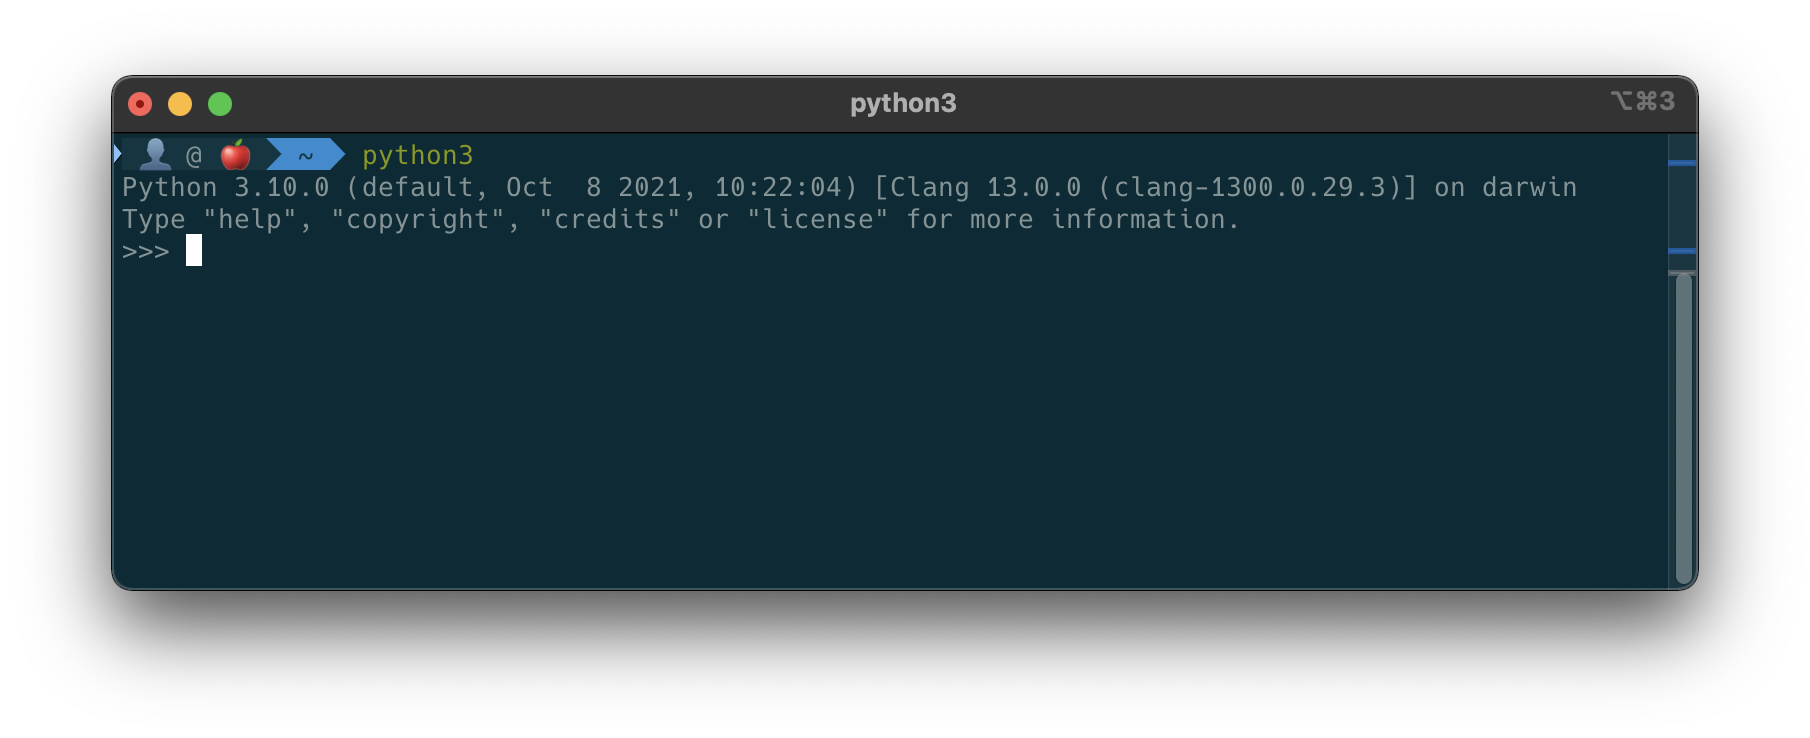
\includegraphics[scale=0.42]{Pictures/chapter04/python_shell.png}
\caption{De \textit{Python} interpreter, met versie $3.10.0$}
\label{fig:interpreter} % Unique label used for referencing the figure in-text
%\addcontentsline{toc}{figure}{Figure \ref{fig:webserver}} % Uncomment to add the figure to the table of contents
\end{figure}

\begin{exercise}
Check of de versie van \textit{Python} die je geïnstalleerd hebt overeen komt met de versie die de interpreter aangeeft.
\end{exercise}

De interpreter is een super handig stukje software, waarin je \textit{Python} code, regel voor regel in kunt typen, zodat je kunt checken of de code doet wat je verwacht. 
\begin{exercise}
Traditiegetrouw begint het leren van een nieuwe programmeertaal altijd met uitvoeren van \textit{Hello world!}. Typ in het scherm het volgende in, en zie wat er gebeurt:
\begin{python}[numbers=none]
print('Hello World!')
\end{python}
Hoeveel regels code zou je hier nodig voor zijn bij de Arduino?
\end{exercise}

\begin{remark}
Als er in dit document een stukje voorbeeld code, de regel begint met '$>>>$', dan wordt deze code ingetypt in de interpreter. De opvolgende regel zonder '$>>>$' is dan de uitvoer van de interpreter. Bijvoorbeeld:
\begin{python}
>>> print('Hello World!')
Hello World!
\end{python}
Elk ander stukje voorbeeld code zullen (gedeeltes van) scripts zijn. 
\end{remark}

\section{Editor}\index{Editor}
Elke regel op deze manier intypen is natuurlijk voor grotere programma's niet ideaal, deze slaan we dan ook op in \textit{Python} scripts (bestanden met als extensie $.py$). Deze kun je in principe gewoon maken in een tekst-editor, maar net als bij de \textit{Arduino} werkt het een stuk fijner in een ontwikkelomgeving. Voor \textit{Python} zijn er een flink scala aan zulke ontwikkelomgevingen (ook wel: IDE's). En je bent uiteraard helemaal vrij om zelf je favoriet daarin te kiezen om de opdrachten gedurende dit vak uit te werken.

Voor de beginners kan ik de IDE \textit{Thonny} aanraden: \url{https://thonny.org/}. \par 
Deze heeft naast een gebruikersvriendelijke interface, ook enkele handige tools aan boord die later van pas gaan komen. Bijkomend voordeel is dat dit programma ook standaard wordt meegeleverd met de \textit{Raspberry Pi}. Tijdens de les zullen de voorbeelden ook worden gegeven aan de hand van \textit{Thonny}.
\begin{exercise}
Installeer een \textit{Python} ontwikkelomgeving.
\end{exercise}

\section{Data Types}\index{Data Types}
Net als in \textit{Arduino C}, zijn in \textit{Python} verschillende datatypes beschikbaar, die de basis vormen van de taal. Zo zijn er gehele getallen (vergelijkbaar met \textit{int}s in \textit{C}):

\begin{python}
>>> x = 3
>>> y = 4
>>> x + y
7
\end{python}
Wat direct opvalt, is dat je in \textit{Python} dus niet hoeft aan te geven welk data type je wilt gebruiken. De taal 'snapt' dit automatisch. De puntkomma aan het eind, die bij \textit{C} elke regel code afsluit, wordt hier niet gebruikt. Verder kun je (op vergelijkbare manier als in \textit{C}) de getallen ook schrijven in binair en hexadecimaal:
\begin{python}
>>> x = 0b101
>>> x
3
>>> y = 0x1A
>>> y
26
\end{python}

Naast gehele getallen zijn er ook uiteraard komma-getallen (vergelijkbaar met \textit{float}s in \textit{C}):
\begin{python}
>>> x = 3.0
>>> y = 4.5
>>> x / y
0.6666666666666666
\end{python}

Ook kent de taal Booleans, die enkel \pyth{True} of \pyth{False} kunnen zijn. Waarmee digitale operaties kunnen worden uitgevoerd (vergelijkbaar met de \textit{bool}s uit \textit{C}):
\begin{python}
>>> a = True
>>> b = False
>>> a and not b
True
\end{python}

\newpage

en voor nu als laatste: \pyth{str}, de \textit{string} waarmee tekst kan worden toegekend aan een variabele. (Vergelijkbaar met de \textit{String}s uit \textit{C}):
\begin{python}
>>> a = 'Hello'
>>> b = "World!"
>>> a + ' ' + b  # Plak beide aan elkaar, met een spatie ertussen.
'Hello World!'
\end{python}
Het maakt bij \pyth{str}s dus ook niet uit of je nu enkele (\pyth{'}) of dubbele (\pyth{"}) aanhalingstekens gebruikt. Verder zie je hier ook voor het eerst een regel commentaar, die je kunt toevoegen na een hekje (\pyth{#}).

\begin{exercise}
\textit{Python} heeft een aantal operatoren voor getallen die bekend voor zullen komen: \pyth{+}, \pyth{-}, \pyth{*} om resp. getallen op tellen, af te trekken en te vermenigvuldigen. Maar kent ook een aantal die wat minder voor de hand liggen. Probeer er achter te komen wat \pyth{%} en \pyth{**} doen.
\end{exercise}

Naast dat het bij \textit{Python} dus niet nodig is om van te voren te specificeren welk datatype je gaat gebruiken voor een variabele, kun je ook variabelen van type laten veranderen gedurende het programma. Dit is voor de leesbaarheid niet aan te bevelen, maar het laat wel zien dat \textit{Python} veel losser om gaat met de verschillende types dan dat we gewend waren met \textit{C}:
\begin{python}
>>> x = 12  # x is nu een int
>>> x
12
>>> x = 'abc'  # En vanaf hier een str
>>> x
'abc'
\end{python}

\section{If/Else statements}\index{If/Else statements}
Een van de meest voorkomende en belangrijke dingen die er gebeurt in een programma, is keuzes maken op basis van condities. In z'n meest eenvoudige manier, doen we dat met een \pyth{if}-statement:
\begin{python}
a = 200
if a > 100:
	print('conditie is True!')
	print('a is groter dan 100')
\end{python}
De \pyth{if}-statement is opgebouwd uit $3$ delen: allereerst het woordje \pyth{if}. Dan gevolgd door een conditie (ook wel expressie genoemd), en uiteindelijk een dubbele punt \pyth{:}. Die conditie is het meest interessant, als daar namelijk \pyth{True} uitkomt worden de volgende regels code uitgevoerd, komt er \pyth{False}, gebeurt er in dit geval niets. 

\begin{remark}
\textbf{Let op:} Ook hier is de schrijfwijze van \textit{Python} weer een stuk compacter dan in \textit{C}: waar je bij die laatste vaak gekrulde haken $\{$, $\}$ ziet, gebruikt \textit{Python} juist inspringing om duidelijk te maken wat bijv. bij een statement hoort. Voor het inspringen gebruik je $4$ spaties of een tab. Dit is dus \textbf{essentieel} voor de werking van je programma! Zie bijv. het volgende voorbeeld:
\begin{python}
a = 200
if a > 100:
	print('conditie is True!')
print('a is groter dan 100')
\end{python}
Hier wordt dus regel $3$ enkel uitgevoerd als \pyth{a>100} is, maar regel $4$ altijd. Let dus goed op bij het inspringen van code!
\end{remark}

De \pyth{if}-statement kan uitgebreid worden met een \pyth{else}-clausule, die uitgevoerd wordt als de conditie \pyth{False} is.
\begin{python}
a = 200
if a > 100:
	print('conditie is True!')
	print('a is groter dan 100')
else:
	print('conditie is False!')
	print('a is kleiner of gelijk dan 100')
\end{python}

\textbf{Tip:} Als je niet zeker van jezelf bent wat er precies uit de conditie komt van je \pyth{if}-statement, kun je hier dus handig gebruik maken van de interpreter:
\begin{python}
>>> a = 200
>>> a > 100
True
\end{python}

Soms wil je meerdere condities checken, dit kan met \pyth{elif} (dit staat voor een samentrekking van \pyth{else if}). Je kan daarvan zoveel als je wil in je \pyth{if}-statement stoppen:
\begin{python}
a = 200
if a > 100:
	print('a is groter dan 100')
elif a == 100:
	print('a is precies 100!')
else:
	print('a is kleiner dan 100')
\end{python}
\begin{exercise}
Typ het bovenstaande over in je editor, sla het op als een \textit{.py} bestand. Probeer het programma te starten (In \textit{Thonny}: Zoek naar de groene play knop, genaamd 'run'). Waar kun je de uitvoer van het programma zien?
\end{exercise}

\section{Input/Output}\index{Input/Output}
Zo'n programma als hierboven, die afhankelijk van de waarde van een vast getal iets uitvoert is natuurlijk niet superspannend. Het wordt al interessanter als je input van de gebruiker van het programma kunt vragen. Dat doe je met de functie \pyth{input()}:
\begin{python}
print('Typ iets: ')
a = input()
print('Je typte: ' + a)
\end{python}

\begin{remark}
\textbf{Tip:} Regel $1$ en $2$ zijn ook te combineren tot \pyth{a = input('Typ iets: ')}.
\end{remark}

\begin{exercise}
Voer het bovenstaande stuk code uit. Merk op dat halverwege het programma wordt gepauzeerd. Wat moet je doen om het programma weer verder te laten gaan?
\end{exercise}

\begin{remark}
\textbf{Tip:} In plaats van regel $3$, kun je ook gebruik maken van de zogeheten \textit{f-strings}. Dit is een wat efficiëntere manier van schrijven, maar doet precies hetzelfde: 
\begin{python}
print(f'Je typte: {a}')
\end{python}
Vooral bij langere wat langere strings, kan dit de leesbaarheid van je code bevorderen.
\end{remark}

\newpage 

\section{Huiswerkopdrachten}\index{Huiswerkopdrachten}
\vspace{2mm} 
\begin{exercise} \label{exc4:exc1}
Maak een programma dat de gebruiker om zijn naam vraagt. Groet hierna de gebruiker in de vorm van \textit{"Hallo, <naam>!"}.
\end{exercise}

\begin{exercise}
Breid het programma van opdracht \ref{exc4:exc1} uit, zodat het programma je schreeuwend begroet: \textit{"HALLO, <NAAM>!"}. 

\textbf{Tip:} Zoek zelf uit hoe je een string naar hoofdletters kunt om te zetten, kijk gerust op \href{https://www.w3schools.com/python/python_ref_string.asp}{deze link} om te zien welke functies je op een string kunt uitvoeren.
\end{exercise}

\begin{exercise}
Schrijf een programma dat de gebruiker vraagt om de straal ($r$) van een cirkel in te typen. Geef daarna de omtrek (= $2*r*\pi$) en de oppervlakte (= $r^2*\pi$) op basis van de straal. 

\textbf{Tip 1:} Alles wat de gebruiker intypt, en je afvangt met \pyth{input()} is van het type string. Om van een string met cijfers, een daadwerkelijk getal te maken, gebruik je de functie \pyth{int()}. Bijv. \pyth{x = int('123')}.

\textbf{Tip 2:} Zet bovenin je programma \pyth{import math}, je hebt daarna toegang tot allerlei wiskundige functies. Zo ook \pyth{math.pi} en \pyth{math.pow()}.
\end{exercise}

\begin{remark}
\textbf{Tip:} Als je niet zeker van jezelf bent wat voor type een variabele krijgt, kun je ook hier handig gebruik maken van de interpreter en de functie \pyth{type()}:
\begin{python}
>>> a = 'een string'
>>> b = 4
>>> type(a)
<class 'str'>
>>> type(b)
<class 'int'>
\end{python}
\end{remark}

\begin{exercise}
Breid het programma van opdracht \ref{exc4:exc1} uit, zodat het programma de gebruiker vraagt om achtereenvolgens z'n voornaam, achternaam, geslacht en leeftijd. 

Groet hierna de gebruiker in de vorm \textit{"Hallo, <voornaam>!"}. 

Is de persoon in kwestie echter ouder dan $50$, gebruik dan een formelere begroeting op basis van zijn of haar geslacht: \textit{"Gegroet, Mr. <achternaam>!"} of \textit{"Gegroet, Mevr. <achternaam>!"}
\end{exercise}

\begin{exercise}
Maak een programma dat de gebruiker vraagt om een getal, geef daarna aan of dat getal even of oneven is.
\end{exercise}

\begin{exercise}
Schrijf een programma dat de gebruiker vraagt om 2 getallen in te voeren, print daarna de grootste van de twee op het scherm. 
\end{exercise}

\begin{exercise}
Schrijf een programma dat de gebruiker vraagt om een getal. Dit getal correspondeert met een dag in de week ($1$ = maandag, $2$ = dinsdag, etc.). print de correspondeerde dag op het scherm. Als de gebruiker een getal groter dan $7$ of kleiner dan $1$ invoert, geef dan een 'error'.
\end{exercise}


\chapter{Python op de Pi}

\section{Introductie linux terminal}\index{Introductie linux terminal}

\section{Editor}\index{Editor}

\section{Pi header}\index{Pi header}

\section{GPIO}\index{GPIO}

\section{Loops}\index{Loops}
Als we bepaalde onderdelen van onze code vaker uit willen voeren, kunnen we dat doen aan de hand van \textit{loops}. In \textit{C} hadden we al kennisgemaakt met de \pyth{for}-loop. Deze zit gelukkig ook in \textit{Python}, maar werkt wel een beetje anders. We gebruiken deze vaak in combinatie met de funtie \pyth{range()}:
\begin{python}
for x in range(0, 10, 1):
	print(x)
\end{python}
In het bovenstaande voorbeeld roepen we de functie \pyth{range()} aan met 3 argumenten. De eerste geeft het startgetal voor $x$ aan, de tweede bij welke waarde van $x$ de loop moet stoppen, en de derde en laatste met welke hoeveel we $x$ we moeten verhogen bij elke nieuwe iteratie. Dit voorbeeld print dus de getallen $0$ t/m $9$ op het scherm. 

\begin{remark}
De functie \pyth{range()} kun je op $3$ verschillende manieren aanroepen:
\begin{enumerate}
\item[-] \pyth{range(stop)}: Met enkel $1$ argument, de stop waarde. $start=0, step=1$.
\item[-] \pyth{range(start, stop)}: Met $2$ argumenten, voor start en stop. $step=1$.
\item[-] \pyth{range(start, stop, stap)}: En $3$, zoals in het voorbeeld.
\end{enumerate}
In het bovenstaande stukje voorbeeldcode kan dus \pyth{range(0, 10, 1)} worden vervangen door \pyth{range(10)}, want die levert dezelfde functionaliteit.
\end{remark}

Als tweede voorbeeld een loop die van $2$ t/m $25$ loopt, met stapjes van $3$:
\begin{python}
for x in range(2, 25, 3):
	print(x)
\end{python}
Dit print het volgende uit: $2, 5, 8, 11, 14, 17, 20, 23$. De \pyth{for}-loop stopt na $23$, omdat $23+3 = 26$, wat hoger is dan $25$, de stop waarde.


\section{Huiswerkopdrachten}\index{Huiswerkopdrachten}
\begin{exercise}
$\\$
\end{exercise}

\begin{exercise}
$\\$
\end{exercise}

\begin{exercise}
$\\$
\end{exercise}

\begin{exercise}
$\\$
\end{exercise}

\begin{exercise}
$\\$
\end{exercise}

\begin{exercise}
$\\$
\end{exercise}

\begin{exercise}
$\\$
\end{exercise}

\begin{exercise}
$\\$
\end{exercise}


\chapter{Week 4: Diepere duik}
Deze week gaan kijken naar enkele concepten die ons leven als programmeur een stukje makkelijker kunnen gaan maken. We gaan eerst een blik werpen op verzamelingen in de vorm van \textit{lijsten}. Daarna de robuustheid van onze code aanzienlijk verbeteren met \pyth{Try} / \pyth{Except}-blokken en ten slotte meer structuur aanbrengen met de introductie van \textit{functies}. 
% , \textit{Dictionaries} en \textit{tuples}

\section{Lijsten}\index{Lijsten}
De lijsten in \textit{Python} zijn vergelijkbaar met de array's in \textit{C}, maar dan veel flexibeler in te zetten. Het voordeel van een lijst te gebruiken, is dat je data die bij elkaar hoort mooi kunt groeperen. Maar je kunt ook handige operaties op een lijst uitvoeren, zo kun je 'm bijvoorbeeld sorteren, omkeren, of elementen eruit filteren. Eerst gaan we kijken naar het aanmaken ervan, hieronder volgen een aantal willekeurige lijsten:

\begin{python}
# Lijsten met getallen:
cijfers = [1, 2, 3, 5, 10, 15] 
frac = [0.5, 0.25, 0.2, 0.1, 0.001, 0.0005] 

# Lijsten met strings:
namen = ['Piet', 'Jan', 'Klaas']
dagen = ['ma', 'di', 'wo', 'do', 'vr', 'za', 'zo']

# Een lijst met verschillende datatypes in een, kan ook:
mix = [13, 'robotica', 3, 2, 'analyse', 3.14, cijfers]
\end{python}

Lijsten hebben zoals je hierboven kunt zien een naam en een verzameling aan elementen. De elementen staan tussen de blokhaken $[\ ]$, en zijn gescheiden door een komma. Lijsten kunnen elk data type bevatten (er kunnen zelfs verschillende datatypes - en dus ook weer lijsten - in een lijst staan, wat we verder in dit vak niet meer gaan behandelen).

\newpage

Lijsten zijn bijv. heel krachtige dingen om in te zetten in combinatie met \pyth{for}-loops:
\begin{python}
kleuren = ['geel', 'rood', 'groen', 'oranje']

for kleur in kleuren:
	print(f'He, nu issie weer {kleur}!')
\end{python}

In deze \pyth{for}-loop worden alle elementen van \textit{kleuren} een voor een opgeslagen in de variabele \textit{kleur} (regel $3$). En die wordt dan weer gebruikt op regel $4$. De output van het bovenstaande stukje code is als volgt:

\begin{python}
He, nu issie weer geel
He, nu issie weer rood
He, nu issie weer groen
He, nu issie weer oranje
\end{python}

Zoals is gezegd, zijn er een aantal handige operaties uit te voeren op een lijst:
\begin{python}
>>> a = [3,2,4,1]
>>> len(a)
4
>>> a.append(5)
>>> a
[3, 2, 4, 1, 5]
>>> len(a)
5
>>> a.reverse()
>>> a
[5, 1, 4, 2, 3]
>>> a.sort()
>>> a
[1, 2, 3, 4, 5]
\end{python}

\begin{exercise}
Maak zelf een lijst aan. Ga na wat de functies \pyth{count()}, \pyth{pop()} en \pyth{remove()} doen. 
\end{exercise}

% \section{Tuples}\index{Tuples}

% \section{Dictionaries}\index{Dictionaries}

\section{Try ... Except}\index{Try ... Except}
Je bent ze inmiddels ongetwijfeld tijdens het maken van de huiswerkopdrachten (of elders) tegengekomen: \textit{errors}. Bijv. bij het opvragen van gegevens bij de gebruiker, via de \pyth{input()}-functie:
\begin{python}
x = input('Geef een cijfer: ')
x = int(x)  # Zet de input-string om naar een int, en sla dit weer op in 'x'.
x += 1  # Tel er 1 bij op
print(f'Een hoger: {x}')
\end{python}
Deze code runt doorgaans prima:
\begin{python}
Geef een cijfer: 12
Een hoger: 13
\end{python}
Maar wat nu als de gebruiker iets verkeerds intypt? Bijv. een letter:
\begin{python}
Geef een cijfer: q
Traceback (most recent call last):
  File "/Users/stefan/Code/Python/err_test.py", line 2, in <module>
    x = int(x)  # Zet de input-string om naar een int, en sla dit weer op in 'x'.
ValueError: invalid literal for int() with base 10: 'q'
\end{python}
Dan krijg je dus een \textit{error} voor je kiezen, in dit geval een \pyth{ValueError}. Bijkomend nadeel: het programma sluit direct af (crasht). Gelukkig geeft \pyth{Python} bij errors vaak genoeg informatie waarmee je de bug je in je code kunt oplossen. Hierboven kun je lezen dat er iets mis gaat op regel $2$: \pyth{x = int(x)}, op het moment dat we de \pyth{str} $q$ om proberen te zetten naar een \pyth{int}. En dat is best te verklaren natuurlijk, $q$ is domweg geen getal. 

\begin{remark}
\textbf{Tip: } Mocht je nu op zoek zijn naar de \textit{ASCII}-waarde van een karakter, gebruik dan de \pyth{ord()}-functie:
\begin{python}
>>> ord('a')
97
>>> ord('b')
98
\end{python}
\end{remark}

Een gebruiker kan nou eenmaal iets verkeerds intypen en het zou vrij suf zijn als dan elke keer je programma crasht. Vandaar dat er in \textit{Python} functionaliteit zit om dit soort fouten van buitenaf af te vangen en op te reageren. Dit doen we door onze kritische code (in dit geval het omzetten van een \pyth{str} naar een \pyth{int}: \pyth{x = int(x)}) in een \pyth{try} / \pyth{except} blok te zetten. En dat ziet er als volgt uit:

\begin{python}
x = input('Geef een cijfer: ')
try:
	x = int(x)  # Zet de input-string om naar een int, en sla dit weer op in 'x'.
	x += 1  # Tel er 1 bij op
	print(f'Een hoger: {x}')
except ValueError:
    print('Dat was geen getal, probeer het nog eens')
\end{python}

Hier 'proberen' we de \pyth{str} te interpreteren als een \pyth{int}. Gaat dat goed, dan wordt er netjes de rest van de code uitgevoerd. Krijg je een error, dan wordt het stuk code na de \pyth{except} uitgevoerd, en wordt de gebruiker vriendelijk verzocht 'even normaal te doen' en het nog eens te proberen. \newline

Elke error die je tegenkomt kun je op deze manier afvangen. Let daar wel bij op, dat niet elke error afgevangen hoeft te worden. Fouten die je zelf als programmeur maakt horen daar vaak niet bij, het gaat meer om fouten van 'buitenaf'. Bijv. je probeert connectie te maken met een server, maar die is op het moment uit de lucht. Dan zul je wellicht iets in de trant van een \pyth{ConnectionError} of een \pyth{TimeOutError} krijgen, die zijn handig om af te vangen. Je wilt niet dat door iets van buitenaf je programma crasht. Voor de liefhebber: hier is een lijstje te zien van de errors die standaard te vinden zijn in \textit{Python}: \url{https://docs.python.org/3/library/exceptions.html}.

\newpage

\section{Functies}\index{Functies}
\textit{Functies} waren we ook al tegengekomen in \textit{C}, in \textit{Python} is de opzet ervan hetzelfde: Een blok aan code, die alleen wordt uitgevoerd als de functie wordt 'aangeroepen'. Je maakt ze aan ('definieert' ze) met \pyth{def}, zie ook het onderstaande voorbeeld:

\begin{python}
def my_function():
    print('Hallo vanuit een functie!') 

my_function()
print('Hallo vanuit het hoofdprogramma!')
my_function()
\end{python}

Dit produceert de volgende output:

\begin{python}
Hallo vanuit een functie!
Hallo vanuit het hoofdprogramma!
Hallo vanuit een functie!
\end{python}

Je ziet in het programma op de eerste $2$ regels de gemaakte functie, na het woordje \pyth{def}. De naam van de functie is \textit{my\_function}, alle regels die daarna volgen en ingesprongen zijn (tab), horen bij deze functie. 
In dit geval is dit maar $1$ regel, namelijk een \pyth{print()}. \newline

Daarna wordt deze functie 'aangeroepen', dat gebeurt voor het eerst op regel $4$. Dat doe je dus door de naam van de functie te typen, gevolgd door $2$ haakjes $( )$. Even later op regel $6$ gebeurt hetzelfde nog eens. \newline

Dit was een voorbeeld van een functie zonder argumenten. Vaak zul je ook functies zien en maken die dat juist wel hebben. Een argument is iets wat je meegeeft met de functie. Dat kunnen er zoveel zijn als je wilt, en ook van elk datatype. Hieronder een voorbeeld met $2$ argumenten, van het type \pyth{str}:

\begin{python}
def my_function(naam, vraag):
    print(f'Hallo {naam}! {vraag}?') 

my_function('Henk', 'Hoe gaat het')
my_function('Piet', 'Waddup')
\end{python}
De uitoer zal in dit geval zijn:
\begin{python}
Hallo Henk! Hoe gaat het?
Hallo Piet! Waddup?
\end{python}

Valt je op je dat nog steeds nergens het datatype hoeft aan te geven? \textit{Python} snapt dat het om \pyth{str} gaat, omdat je ze als zodanig meegeeft op regel $4$ en $5$. 

\begin{remark}
De functie zal het ook prima doen als je 'm aanroept met bijv. getallen: \newline 
\pyth{my_fucntion(1, 2)}
\begin{python}
Hallo 1! 2?
\end{python}
\textit{Python} gaat heel flexibel met om datatypes. Omdat alles wat in de functie \textit{my\_function} gebeurt met de argumenten \textit{naam} en \textit{vraag} ook prima gedaan kan worden met getallen, krijg je geen errors. In \textit{C} vlogen nu de errors en warnings om je oren.
\end{remark}

\newpage

Dan rest ons nog een ding om in te duiken, functies die iets teruggeven. Het kan zijn dat een functie een bepaalde operatie uitvoerd, en dat je het resultaat daarvan graag wil gebruiken verderop in je programma. Dat kan, net als in \textit{C} met \pyth{return}. Zie ook het volgende voorbeeld:

\begin{python}
import math 

def oppervlakte(r):
    # Berekend de oppervlakte van een cirkel ahv de straal.
    opp = r**2 * math.pi
    return opp

o5 = oppervlakte(r=5)
print(f'Oppervlakte cirkel, bij straal=5:  {o5}')

o10 = oppervlakte(10)
print(f'Oppervlakte cirkel, bij straal=10: {o10}')

print(f'Oppervlakte cirkel, bij straal=15: {oppervlakte(15)}')

o20 = oppervlakte(20)
print(f'Oppervlakte cirkel, bij straal=20: {o20:.2f}')
\end{python}

In tegenstelling tot \textit{C} hoef je ook hier geen datatype op te geven, dat wordt voor je geregeld. Enkel de functie afsluiten met een \pyth{return}-statement is voldoende om de functie een waarde terug te laten geven. \newline


De functie \pyth{oppervlakte()} berekend de oppervlakte van een cirkel a.h.v. de meegegeven straal \pyth{r}. En hij wordt op vier verschillende manieren aangeroepen:
\begin{enumerate}
	\item[-] Allereerst op regel $8$ met een straal van $r=5$, hier wordt ook de naam van het argument ($r$) meegegeven, dat leest makkelijker, maar is niet nodig. Het antwoord van de functie wordt opgeslagen in variabele $o5$ en naar het scherm gescreven. \newline

	\item[-] Daarna wordt de functie aangeroepen met een straal van $r=10$, het antwoord hiervan wordt daarna opgeslagen in de variabele $o10$, die dan geprint wordt op het scherm. \newline

	\item[-] Daarna op regel $14$, wordt het aanroepen van de functie (met $r=15$) en het printen van de teruggegeven waarde gecombineerd tot een regel code. \newline

	\item[-] En tenslotte wordt de functie nog een keer aangeroepen voor $r=20$ op regel $16$. Bij het printen (regel $17$) gebeurt iets bijzonders, daar wordt namelijk aangegeven dat de uitvoer maar $2$ kommagetallen moet laten zien (dit komt door de \pyth{:.2f} in \pyth{print}). 
\end{enumerate}

De uitvoer van het programma is dan ook:
\begin{python}
Oppervlakte cirkel, bij straal=5:  78.53981633974483
Oppervlakte cirkel, bij straal=10: 314.1592653589793
Oppervlakte cirkel, bij straal=15: 706.8583470577034
Oppervlakte cirkel, bij straal=20: 1256.64
\end{python}

\newpage
Zoals ik vorige week stelde, kun je met functies in combinatie met de \pyth{gpiozero}-module leuke dingen doen. Zo kun je dus bijv. functies aanroepen, als er een bepaalde actie wordt uitgevoerd word, zoals het indrukken en het loslaten van een knop:
\begin{python}
from gpiozero import Buttons
from signal import pause

def ingedrukt():
	print('knop ingedrukt!')

def losgelaten():
	print('knop weer losgelaten!')

btn = Button(2)  # Drukknop zit op GPIO2

btn.when_pressed = ingedrukt    # Koppel functie bij het indrukken.
btn.when_released = losgelaten  # Koppel functie bij het loslaten.
pause()                         # Doe verder niets meer, maar sluit niet af.
\end{python}

\begin{exercise}
Voor het programma uit, en ga voor jezelf na wat er precies gebeurt.
\end{exercise}

\begin{remark}
Weet je nog uit Programmeren $1$, dat knoppen last kunnen hebben van het zogeheten \textit{bouncen}, waardoor het lijkt dat ze veel vaker ingedrukt worden, dan ze daadwerkelijk worden. Mocht je daar nu ook last van hebben, dan kun je met \pyth{gpiozero} vrij makkelijk de bounce-tijd instellen. Vervang regel $10$ door:
\begin{python}
# Drukknop zit op GPIO2 met 100ms bounce time:
btn = Button(2, bounce_time=0.1)  
\end{python}
\end{remark}

De laatste regel \pyth{pause()}, zorgt dat het programma verder niets meer uitvoert, (behalve het afhandelen van de knop) maar ook niet afsluit. In tegenstelling tot de \pyth{while True:} uit het vorige hoofdstuk, waardoor de \textit{Raspberry Pi} intensief gebruikt werd, kan hij in dit geval rustig andere taken doen. 

\begin{remark}
Het mooie van het kunnen koppelen van functies aan gebeurtenissen van een sensor (zoals hier in het geval van de drukknop), is dat dat ook functies kunnen zijn die gebruikt worden door actuatoren, zoals bijv. een LED. Een LED heeft een \pyth{on()}- en een \pyth{off()}-functie. Dus het koppelen van een LED aan een drukknop kan zo:

\begin{python}
from gpiozero import Buttons, LED
from signal import pause

btn = Button(2)  # Drukknop zit op GPIO2
led = LED(17)    # LED zit op GPIO17

# Koppel het indrukken van de knop met led.on():
btn.when_pressed = led.on    
# Koppel het loslaten van de knop met led.off():
btn.when_released = led.off  

# Doe verder niets meer, maar sluit niet af:
pause()                      
\end{python}
\end{remark}

\newpage
Afsluitend aan dit hoofdstuk gaan we eens wat dingen combineren die we geleerd hebben. Je kunt namelijk elementen uit een lijst filteren, als je daarvoor een filter-functie voor aanmaakt. Bijv. je hebt een bepaalde temperatuursensor, waar je elk uur de temperatuur mee meet, maar deze geeft af en toe een foute waarde (bijv. +$100^\circ C$ op een winterdag). 

\begin{python}
def temp_filter(temp):
    # Filter-functie, voor temp groter dan 90 graden.
    if (temp > 90):
        return False
    else:
        return True

# Lijst met gemeten temperatuur in celcius:  
gemeten_temp = [15.2, 14.4, 14.2, 99.9, 13.8, 12.6, 100.1]

# Pas filter toe:
gefilterde_temp = filter(temp_filter, gemeten_temp)

# Print de overgebleven waardes op het scherm:
print('De gefilterde temperaturen zijn:')
for t in gefilterde_temp:
    print(t)                    
\end{python}

In het bovenstaande voorbeeld, wordt een filter-functie aangemaakt \pyth{temp_filter(temp)}. Die een \pyth{False} teruggeeft als de meegegeven temperatuur \pyth{temp} groter is dan $90$, en anders \pyth{True}. \newline

Op regel $12$ wordt die filterfunctie daadwerkelijk toegepast op de lijst \pyth{gemeten_temp} en de nieuwe lijst die dat opleverd wordt opgelsagen in \pyth{gefilterde_temp}

\newpage

\section{Huiswerkopdrachten}\index{Huiswerkopdrachten}

\begin{exercise}\label{exc6:exc1}
Maak een lege lijst aan, en vul deze daarna met de getallen $1$ t/m $100$.
Gebruik hiervoor een loop en de \pyth{append()} functie. \newline
\textbf{Tip:} Een lege lijst maak je als volgt aan: \pyth{lijst = []}
\end{exercise}

\begin{exercise}
Maak een filter-functie waarmee je alle getallen onder de $30$ uit een lijst kunt filteren. Pas deze toe op de lijst die je gemaakt hebt bij opdracht \ref{exc6:exc1}.
\end{exercise}

\begin{exercise}
Maak een filter-functie waarmee je oneven getallen uit een lijst kunt filteren. Pas deze toe op de lijst die je gemaakt hebt bij opdracht \ref{exc6:exc1}.
\end{exercise}

\begin{exercise}
\label{exc6:exc4}
Maak een functie \pyth{schreeuw} die een meegegeven str omzet naar hoofdletters, en deze daarna weer terug geeft met \pyth{return}. 
\end{exercise}

\begin{exercise}
Wat als je nu de functie die net gemaakt hebt bij \ref{exc6:exc4}, aanroept met een getal (bijv. \pyth{schreeuw(5)})? \newline
Breidt de functie uit met een \pyth{try} / \pyth{except}, zodat deze niet langer crasht. 
\end{exercise}

\begin{exercise}
Sluit $4$ LEDs aan op de \textit{GPIO17}, \textit{GPIO18}, \textit{GPIO3} en \textit{GPIO5} pins. Configureer ze, en zet ze daarna in een lijst. Ga met een loop door de lijst heen, en zet ze een voor een $1$ seconde aan, en dan weer uit.
\end{exercise}

\begin{exercise}
Maak een programma die $10$ keer aan de gebruiker vraagt om een dier in te voeren. Voeg elk van deze dieren toe aan een lijst. Filter alle diernamen die minder dan $3$ letters hebben en print daarna de lijst in alfabetische volgorde op het scherm. \newline
\textbf{Tip:} Je bepaalt de lengte van een string (of lijst) met de functie: \pyth{len(mijn_string)}.
\end{exercise}

\chapter{Week 5: Data-analyse in Python}

We hebben inmiddels een gedegen bassis kennis van \textit{Python} opgedaan gedurende dit vak. We hebben o.a. geleerd over loops, lijsten, functies en IO aansturing in \textit{Python}, en de vershillen gezien met \textit{C}. Een van de concepten die nog onbelicht is gebleven is het zogeheten 'object georiënteerd programmeren' (of \textit{OOP}).
Omdat dit een van de belangrijkste en handigste concepten van het programmeren is van de afgelopen decenia, én omdat we stiekem er toch al flink mee gewerkt hebben, gaan we in dit hoofdstuk ook dit thema belichten. Daarnaast gaan we deze week aan de slag met \textit{packages}, handige software bibliotheken die de functionaliteit van onze \textit{Python} omgeving kunnen uitbreiden. 

\section{Object georiënteerd programmeren}\index{Object georiënteerd programmeren}


\section{Packages}\index{Packages}
Een \textit{Package} in \textit{Python} is een verzameling van modules. Deze modules kunnen we weer in onze code gebruiken door deze te importeren met \pyth{import}. We hbben er in middel al een aantal van gebruikt bijv.: \pyth{math, time, gpiozero, RPi}, maar deze worden allemaal standaard meegeleverd. Je kunt ze ook heel eenvoudig zelf toevoegen aan je \textit{Python} omgeving, door gebruik te maken van \pyth{pip}. Dit programma kun je aanroepen vanaf de terminal:
\begin{lstlisting}[language=bash]
python3 -m pip install <naam_package>
\end{lstlisting}

\begin{remark}
Je hebt ongetwijfeld al een hele lijst geïnstalleerd zonder dat je het wist, je kunt het bekijken door het onderstaande in een terminal in te typen: 
\begin{lstlisting}[language=bash]
python3 -m pip list
\end{lstlisting}
En als je wat schijfruimte wilt vrij maken door packages te verwijderen die je niet langer gebruikt, kan dat met:
\begin{lstlisting}[language=bash]
python3 -m pip uninstall <naam_package>
\end{lstlisting}
\end{remark}

Om een beetje bekend te raken met \textit{pip}, gaan we als voorbeeld een kleine package installeren genaamd \pyth{camelcase}:
\begin{lstlisting}[language=bash]
python3 -m pip install camelcase
\end{lstlisting}

Probeer nu het volgende scriptje te draaien:
\begin{python}
from camelcase import CamelCase     # importeer onze nieuwe aanwinst

c = CamelCase()                     # Nodig om de package te kunnen gebruiken.
txt = 'pip onder de knie krijgen!'  # De tekst die omgezet dient te woren.

print(c.hump(txt))                  # Pas camelcase toe op de tekst.
\end{python}
Als dat lukt, is de module juist geïnstalleerd en heb je de basis van \textit{pip} onder de knie! (Deze packages worden overigens gedownload vanaf \url{https://pypi.org/}, kijk er gerust eens na en wellicht kom je er interressante tegen tussen de bijna 350.000 packages.) \\
Het aanpassen van hoofdletters is echter niet al te spannend, dus gaan we verder met een package waar we echt iets aan hebben: \textit{matplotlib}. 
\section{matplotlib}\index{matplotlib}

\begin{figure}[h!]
\centering
\includegraphics[scale=0.25]{Pictures/chapter07/matplotlib_logo.png}
% \caption{\small \textit{Matplotlib} logo. Bron: \url{https://matplotlib.org}}
\label{fig:mpllogo} % Unique label used for referencing the figure in-text
%\addcontentsline{toc}{figure}{Figure \ref{fig:webserver}} % Uncomment to add the figure to the table of contents
\end{figure}

Matplotlib is een verzameling aan tools voor het maken en bewerken van grafieken. 
\begin{exercise}
  Installeer Matplotlib
\end{exercise}

Om het te gebruiken in z'n meest simpele vorm zorg je ervoor dat je een reeks $x$-waardes hebt, en een reeks bijbehorende $y$-waardes. Deze kun je dan plotten (het daadwerkelijk tekenen van de grafiek) en de resulterende grafiek kun je tonen op het scherm:

\inputpython{code/chapter07/plot1.py}

Hieruit rolt grafiek \ref{fig:plot1} uit:
\begin{figure}[h!]
\centering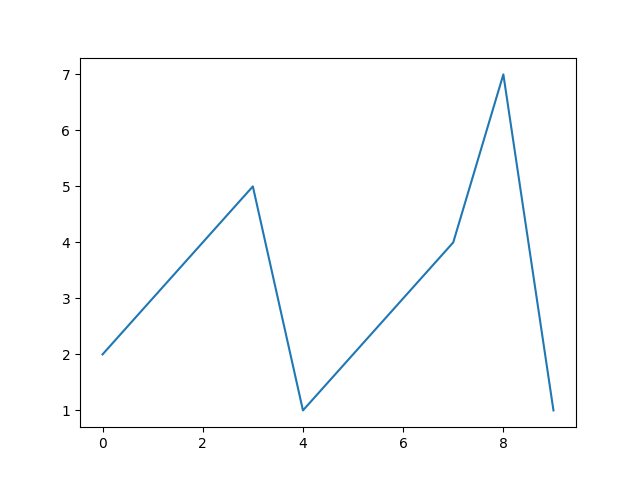
\includegraphics[scale=0.7]{Pictures/chapter07/plot1.png}
\caption{Simpele plot met \textit{Matplotlib}}
\label{fig:plot1} % Unique label used for referencing the figure in-text
%\addcontentsline{toc}{figure}{Figure \ref{fig:webserver}} % Uncomment to add the figure to the table of contents
\end{figure}

\begin{remark}
Kreeg je bij het runnen van bovenstaande code op de \textit{Pi} een error, in de trant van \textit{'Error retrieving accessibility bus address'}? Dan kan het zijn dat je een module in Linux mist, open een terminal en voer in: 
\begin{lstlisting}[language=bash]
sudo apt-get update
sudo apt-get install at-spi2-core
\end{lstlisting}
\end{remark}

Een grafiek is natuurlijk pas echt bruikbaar als deze netjes is opgemaakt met duidelijke labels voor de assen en eventueel een titel en een legenda. Ook dat is snel gepiept met \textit{matplotlib}. In het onderstaande stuk code voegen we dit toe aan ons eerdere script. Daarnaast is er een extra set met $y$-waardes toegevoegd, om $2$ verschillende meetmomenten na te bootsen.

\inputpython{code/chapter07/plot2.py}

De bonenstaande code produceert onderstaande grafiek \ref{fig:plot2}:
\begin{figure}[h!]
\centering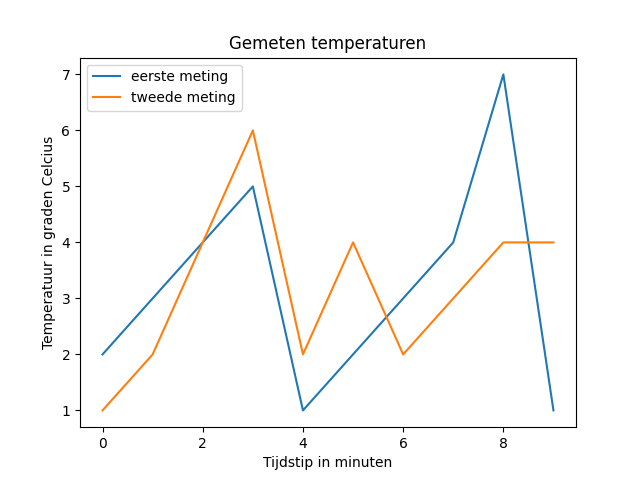
\includegraphics[scale=0.7]{Pictures/chapter07/plot2.png}
\caption{Uitgebreidere plot met \textit{Matplotlib}}
\label{fig:plot2} 
%\addcontentsline{toc}{figure}{Figure \ref{fig:webserver}} % Uncomment to add the figure to the table of contents
\end{figure}

\begin{exercise}
Zorg dat de eerste lijn rood gekleurd (\pyth{color}) wordt, en de tweede lijn groen en gestippeld (\pyth{linestyle}). \\
\textbf{TIP: } Gebruik hiervoor de documentatie van de packge op: \url{https://matplotlib.org}. 
\end{exercise}

\subsection{NumPy}\index{NumPy}

\begin{figure}[h!]
\centering
\includegraphics[scale=0.5]{Pictures/chapter07/numpy_logo.png}
% \caption{\small \textit{Matplotlib} logo. Bron: \url{https://matplotlib.org}}
\label{fig:numpylogo} % Unique label used for referencing the figure in-text
%\addcontentsline{toc}{figure}{Figure \ref{fig:webserver}} % Uncomment to add the figure to the table of contents
\end{figure}

De mogelijkheden van \textit{matplotlib} kunnen enorm uitgebreid worden in combinatie met andere packages. Een voor de hand liggende keuze daarin is bijvoorbeeld \textit{NumPy}. Die een enorm scala aan wiskundige tools met zich meebrengt. 

\begin{exercise}
Installeer NumPy 
\end{exercise}
We kunnen met de combinatie \textit{NumPy} en \textit{matplotlib} bijv. elke wiskunde functie die we kunnen bedenken op een makkelijke en overzichtelijke wijze plotten. Superhandig voor je wiskunde huiswerk ;). Als voorbeeldje volgt hieronder een klein scriptje die $y = sin(x)$ plot op een bereik van $-\pi$ tot $\pi$:
\inputpython{code/chapter07/plot_numpy.py}

De bonenstaande code produceert onderstaande grafiek \ref{fig:plot3}:
\begin{figure}[h!]
\centering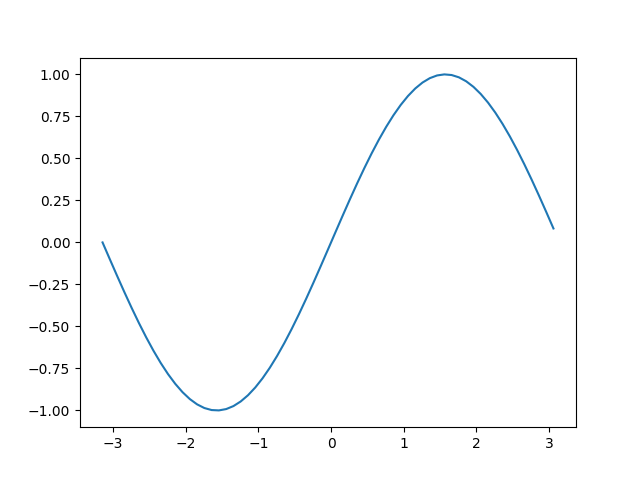
\includegraphics[scale=0.7]{Pictures/chapter07/sin.png}
\caption{Een sinus-functie tekenen met \textit{Matplotlib} en \textit{NumPy}.}
\label{fig:plot3} 
%\addcontentsline{toc}{figure}{Figure \ref{fig:webserver}} % Uncomment to add the figure to the table of contents
\end{figure}

Op regel $5$ wordt hier een reeks aan getallen gegenereerd door de \pyth{np.arange()}-functie. Valt je op dat deze functie nagenoeg hetzelfde eruit ziet (en werkt!) als de ingebouwde \pyth{range()}-functie? Het verschil zit 'm in dat \pyth{np.arange()} ook komma-getallen (floats) kan genereren. \\ 
Om een soortgelijke reden gebruiken we op regel $7$ \pyth{np.sin()} in plaats van \pyth{math.sin()}. De sinus functie uit \textit{NumPy} kan namelijk de sinus van een hele reeks getallen uitrekenen en dit weer teruggeven als een reeks getallen. De sinus-functie uit \pyth{math} kan enkel de sinus uitrekenen op $1$ getal per keer.
 
% \subsection{pip}\index{pip}

\section{Pandas}\index{Pandas}
\begin{figure}[h!]
\centering
\includegraphics[scale=0.2]{Pictures/chapter07/pandas_logo.png}
% \caption{\small \textit{Matplotlib} logo. Bron: \url{https://matplotlib.org}}
\label{fig:pandaslogo} % Unique label used for referencing the figure in-text
%\addcontentsline{toc}{figure}{Figure \ref{fig:webserver}} % Uncomment to add the figure to the table of contents
\end{figure}

% \subsection{Excel file edit}\index{Excel file edit}
Het tekenen van grafieken wordt een stuk intteressanter als je veel input data hebt. Die kun je bijvoorbeeld krijgen door een sensor periodiek te meten, maar ook door een spreadsheet in te laden. De package \textit{pandas} helpt je bij dat laatste enorm.

\begin{exercise}
Installeer de package \textit{Pandas} en z'n verschillende parser:
\begin{lstlisting}[language=bash]
python3 -m pip install pandas odfpy openpyxl xlrd
\end{lstlisting}
De laatste drie packages die hier worden geïnstalleerd zijn resp. nodig voor support van $.ods$- (LibreOffice), $.xslx$- (Microsoft Excel) en $.xls$- (Oude Microsoft Excel) bestanden. Mocht je bepaalde bestandsformaten niet gaan gebruiken, kun je die uiteraard overslaan.
\end{exercise}

Naast de \textit{Python} packages ben je natuurlijk ook een programma nodig dat spreadsheets kan maken en bewerken. Op je laptop gebruik je hier ongetwijfeld Microsoft Excel voor. Voor de Raspberry Pi moet je hier waarschijnlijk nog even een programma voor installeren. Voor een complete office suite variant, kun je bijv. LibreOffice installeren. Dit is een gratis, en een heel complete vervanger voor Microsoft Office (die overigens ook prima draait op je laptop ;) ).\\\\ 
Heb je nu geen zin in een grote download, kun je ook kiezen voor Gnumeric. Dat is gewoon een basic spreadsheet editor zonder poespas, maar wel met alle functionaliteit in huis die we tijdens dit vak nodig zijn.

\begin{exercise}
Installeer op basis van je voorkeur een spreadsheet programma op je Pi:
\begin{lstlisting}[language=bash]
sudo apt-get install libreoffce
\end{lstlisting}
of:
\begin{lstlisting}[language=bash]
sudo apt-get install gnumeric
\end{lstlisting}
\end{exercise}

Als voorbeeld heb ik de volgende spreadsheet aangemaakt: Een tabel met twee kolommen: 'Tijdstip' en 'Waarde', met elk $50$ rijen/waardes. 
\begin{figure}[h!]
\centering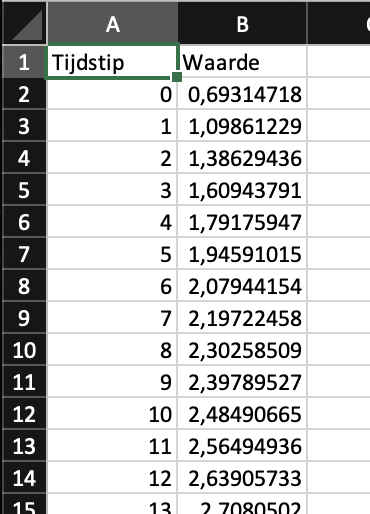
\includegraphics[scale=0.7]{Pictures/chapter07/excel1.png}
\caption{Voorbeeld spreadsheet gemaakt in Excel.}
\label{fig:excel1} % Unique label used for referencing the figure in-text
%\addcontentsline{toc}{figure}{Figure \ref{fig:webserver}} % Uncomment to add the figure to the table of contents
\end{figure}

Deze spreedsheet is dan met \textit{pandas} als volgt heel eenvoudig in te laden:
\inputpython{code/chapter07/exc1.py}

\begin{remark}
Heb je nu een spreadsheet met meerdere tabladen gemaakt en wil je een specifiek blad inladen met de naam 'Blad1'? Dat kan prima. Pas dan regel $5$ aan van de code naar: \\
\pyth{df = pd.read_excel('excel1.xlsx', sheet_name='Blad1')}
\end{remark}

Dit stukje code leest de $.xlsx$-bestand in, en print daarna alle namen van de kolommen op het scherm:
\begin{python}
Tijdstip
Waardes
\end{python}

Deze namen kunnen we daarna gebruiken om de daadwerkelijke data te benaderen en bijvoorbeeld te pringten met \textit{matplotlib}:

\inputpython{code/chapter07/exc2.py}

\newpage

Dit bovenstaande stukje code levert uiteindelijk de volgende grafiek op:

\begin{figure}[h!]
\centering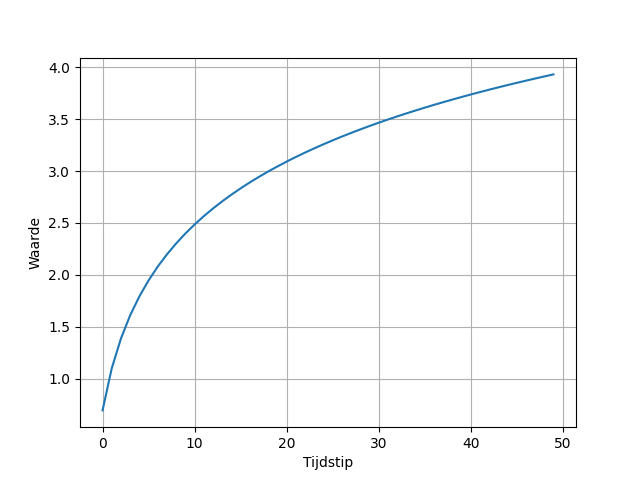
\includegraphics[scale=0.7]{Pictures/chapter07/plot3.png}
\caption{Plot gemaakt vanuit spreadsheet.}
\label{fig:plot3} % Unique label used for referencing the figure in-text
%\addcontentsline{toc}{figure}{Figure \ref{fig:webserver}} % Uncomment to add the figure to the table of contents
\end{figure}

\begin{remark}
Nerdy tip: Je kunt ook in plaats van zelf de x- en y-labels een naam te geven, dit af laten hangen van de gevonden kolomnamen:
\begin{python}
plt.xlabel(df.columns[0])
plt.ylabel(df.columns[1])
\end{python}
\end{remark}

Andersom kan natuurlijk ook: Je hebt data in je \textit{Python} script, en dat wil je opslaan als een spreadsheet. Dat is wat we met het volgende stukje code doen:

\inputpython{code/chapter07/toexc.py}

\newpage

Het gegenereerde bestand kunnen we openen met ons spreadsheet-programma, en zal er dan zo uitzien:

\begin{figure}[h!]
\centering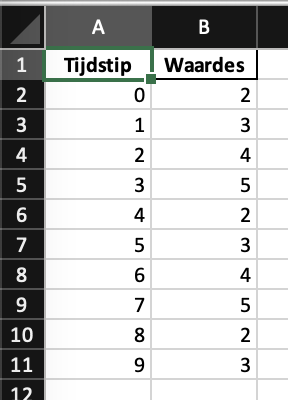
\includegraphics[scale=0.7]{Pictures/chapter07/excel2.png}
\caption{Spreadsheet gegenereerd vanuit \textit{Python}}
\label{fig:excel1} % Unique label used for referencing the figure in-text
%\addcontentsline{toc}{figure}{Figure \ref{fig:webserver}} % Uncomment to add the figure to the table of contents
\end{figure}

\begin{exercise}
Op regel $8$ gebruiken we de \pyth{zip()}-functie. Ga na in de interpreter wat deze functie precies doet met 2 lijsten. 
\end{exercise}

\newpage

\section{Opdrachten}\index{Opdrachten}
\begin{exercise}
Plot (in $1$ grafiek) met \textit{matplotlib} en \textit{NumPy} de functies: \\
$y_{1}=\sin(2\cdot x)$ en $y_{2}=4\cdot\cos(4\cdot x)$ tussen $-2\pi$ en $2\pi$.\\
Zorg ook voor een duidelijke legenda.
\end{exercise}

\begin{exercise}
\label{exc7:exc2}
Vraag van de gebruiker steeds een nummer, net zolang tot deze 'klaar' intypt. 
Voeg alle getallen die de gebruiker intypte steeds toe aan een lijst en print hier een nette grafiek van. (Begin voor de x-waardes te tellen bij $0$, en tel er steeds 1 bij op, voor elk ingevoerd getal).
\end{exercise}

\begin{exercise}
Breid het het programma van opdracht \ref{exc7:exc2} uit, zodat het programma ook een Excel sheet opslaat met alle ingevoerde cijfers.
\end{exercise}

\begin{exercise}
TODO: maak een klasse aan voor een RGB led op basis van RPi.GPIO en 3 verschillende leds
\end{exercise}

\begin{exercise}
$\\$
\end{exercise}

\begin{exercise}
$\\$
\end{exercise}

\begin{exercise}
$\\$
\end{exercise}

\begin{exercise}
$\\$
\end{exercise}


\chapter{Week 6: Arduino met Pi Koppelen}

In deze laatste week van het vak Programmeren 2, gaan we ons eerst nog wat verder verdiepen in de wereld van object geörienteerd programmeren (OOP). Daarnaast stevenen we af op onze eindopdracht van dit vak.

\section{Overerven}\index{Overerven}
Met het vorige hoofdstuk heb je eerste introductie gehad in de wereld van OOP. We hebben op een nieuwe abstracte manier naar problemen gekeken. Ook werd er toen verteld over de voordelen van OOP, zo kon je de code makkelijk onderhouden (je hoeft maar op $1$ plek de klasse-definitie/blauwdruk aan te passen, en overal waar je 'm gebruikt wordt deze verandering overgenomen). Maar ook werd er gesteld dat de gemaakte code eenvoudig uitbreidbaar is, en op dat voordeel hebben we nog niet naar gekeken. Als we nu ons geheugen opfrissen door even te kijken naar de gemaakte \pyth{Cirkel}-klasse:

\inputpython{code/chapter08/cirkel.py}

We hadden een klasse \pyth{Cirkel} gemaakt die als eigenschap z'n straal had, en waarop we de functies \pyth{bereken_oppervlakte()} en \pyth{bereken_omtrek()} op kunnen uitvoeren. We kunnen nu deze klasse-definitie nu ook gebruiken om andere klasse te definiëren die gebasseerd zijn op deze cirkel. \newline 

Als we bijvoorbeeld een klasse willen maken voor een \pyth{Bol} en we gaan hiervoor beredeneren wat zijn eigenschappen en z'n functies zijn. Zul je zien dat deze veel zullen overeenkomen met die van de \pyth{Cirkel}. Qua eigenschappen kunnen we een bol definieren op basis van een straal en op basis van die straal kunnen we de omtrek, oppervlakte en inhoud van de bol berekenen. Grafisch weergegeven:
\begin{figure}[h!]
\centering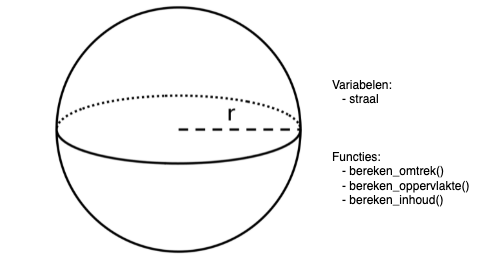
\includegraphics[scale=0.7]{Pictures/chapter08/bol.png}
\caption{\small Ons bol-object heeft een straal, en kan (op basis daarvan) de omtrek, oppervlakte en inhoud van zichzelf berekenen.}
\label{fig:bol} % Unique label used for referencing the figure in-text
%\addcontentsline{toc}{figure}{Figure \ref{fig:webserver}} % Uncomment to add the figure to the table of contents
\end{figure}

Zowel de klasse-variabele \pyth{r}, als $2$ van de $3$ functies\footnote{Wellicht heb je 'm al door: de oppervlakte van een bol berekenen je op een andere manier dan van een cirkel, hier komen we later op terug} komen overeen met die van \pyth{Cirkel}. Als we dus een klasse-definitie voor een \pyth{Bol} willen maken is het handiger om deze te baseren op \pyth{Cirkel} dan helemaal opnieuw te beginnen, dat scheelt werk! Onze klasse-definitie van een \pyth{Bol} ziet er dan zo uit:

\inputpython{code/chapter08/bol.py}

Valt het je op hoe kort dit bestand is? Op regel $5$ gebeurt alle 'magie', hier wordt namelijk gesteld dat we een nieuwe klasse genaamd \pyth{Bol} willen maken, maar dat we deze willen baseren op \pyth{Cirkel}. \textit{Python} regelt nu onderwater dat de bol-klasse een klasse-variabele \pyth{r} voor de straal krijgt, en ook kan hij gebruik maken van de functies (waaronder de constructor) die in \pyth{Cirkel} zitten. \newline

Het enige wat wij zelf nog moeten doen is de nieuwe functie uitschrijven die de inhoudt van de bol berekend op basis van z'n straal, met de volgende formule: $V_{bol} = \frac{4}{3} \pi r^3$. \newline

\begin{remark}
  Een klasse basseren op een andere klasse noemen we ook wel een \textit{subklasse} maken. \pyth{Bol} is in dit geval een \textit{subklasse} van \pyth{Cirkel}. Andersom is \pyth{Cirkel} de \textit{superklasse} van \pyth{Bol}.
\end{remark}

Deze klasse-definitie kunnen we daarna gebruiken in andere programma's op de bekende manier:
\begin{python}
from bol import Bol

mijn_bol = Bol(10)  # Maak een bol aan met een straal van 10.

omt = mijn_bol.bereken_omtrek()
opp = mijn_bol.bereken_oppervlakte()
inh = mijn_bol.bereken_inhoud()

print(f"Omtrek: {omt:.2f}")
print(f"Oppervlakte: {opp:.2f}")
print(f"Inhoud: {inh:.2f}")
\end{python}

Wat het onderstaande als uitvoer geeft:
\begin{python}
Omtrek: 62.83
Oppervlakte: 314.16
Inhoud: 4188.79
\end{python}

We maken hier een object genaamd \pyth{mijn_bol} aan, die van het type \pyth{Bol} is. Doordat onze Bol klasse-definitie geen constructor heeft, wordt de constructor van z'n superklasse aangeroepen: die van \pyth{Cirkel}. Daarna worden de functies \pyth{bereken_omtrek()} en \pyth{bereken_oppervlakte()} aangeroepen. Deze zijn ook niet te vinden in de \pyth{Bol} klasse-definitie, dus worden die van \pyth{Cirkel} hier uitgevoerd. De laatste functie \pyth{bereken_inhoud()} is wel te vinden in \pyth{Bol}, dus die wordt aangeroepen zoal we gewend zijn. \newline

Python zoekt dus eerst in de klasse-definitie van een subklasse naar klasse-variabelen en functies, en als ze daar niet te vinden zijn kijkt hij naar de superklasse ervan. (zijn ze daar ook niet vinden, dan krijg je een \pyth{AttributeError} ;) ). \newline

In onze \pyth{Bol} zit echter nog wel een bug, de oppervlakte van een bol, bereken je op een andere manier dan van een cirkel. Voor een cirkel geldt: $O_{cirkel} = \pi r^2$, voor een bol: $O_{bol} = 4\pi r^2$. \newline

Gelukkig kunnen we in een subklasse functies van de superklasse makkelijk overschrijven:
\inputpython{code/chapter08/bol2.py}

Als we nu onze \pyth{Bol} gebruiken, zoals boven aan deze pagina, komen er wel de juiste waardes uit:
\begin{python}
Omtrek: 62.83
Oppervlakte: 1256.64
Inhoud: 4188.79
\end{python}

In dit geval zoekt Python eerst naar de functie \pyth{bereken_oppervlakte()} in \pyth{Bol}, en vindt 'm daar al, hij zoekt dan niet meer verder. Op deze manier kun je dus functies 'vervangen' van de superklasse in de subklasse. \newline \newline

We doen nog een voorbeeldje. Want we kunnen het overerven ook andersom benaderen. Stel je voor je wil op een OOP manier een kat, een hond en een koe beschrijven. In dit voorbeeld heeft elk dier een aantal variabelen en een aantal functies: 

\begin{figure}[h!]
\centering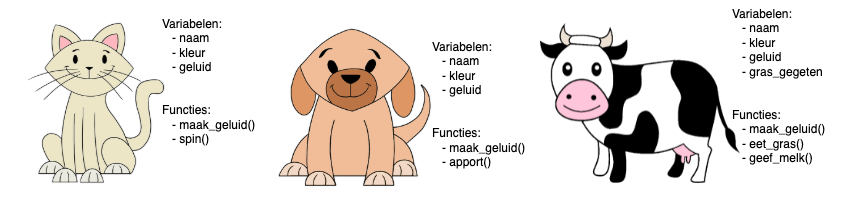
\includegraphics[scale=0.5]{Pictures/chapter08/animals.png}
  \caption{\small Elk dier (kat, hond en koe) heeft z'n eigen eigenschap en functies.} 
\label{fig:animals} % Unique label used for referencing the figure in-text
%\addcontentsline{toc}{figure}{Figure \ref{fig:webserver}} % Uncomment to add the figure to the table of contents
\end{figure}

Deze zou je nu los van elkaar gaan uit kunnen werken in code, maar je kunt ook eerst kijken naar de overeenkomsten. Deze overeenkomsten zou je namelijk kunnen verzamelen in een basis superklasse (bijv. 'dier') , waarop je de andere dieren op basseert. \newline

\begin{figure}[h!]
\centering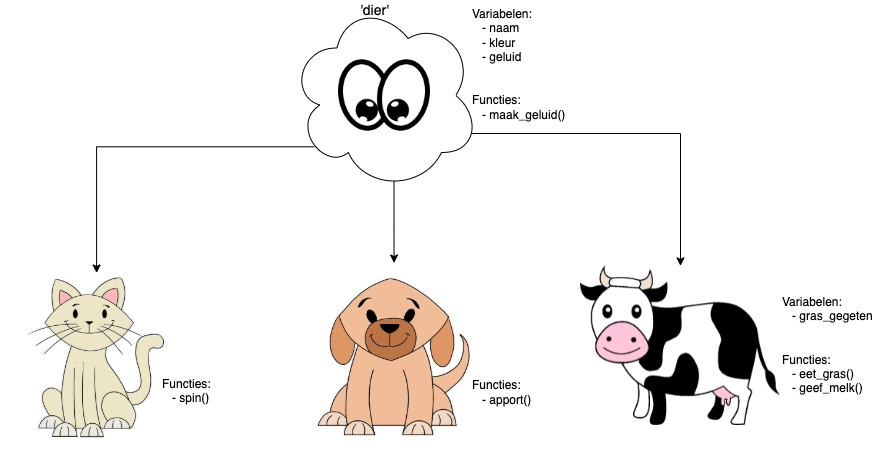
\includegraphics[scale=0.5]{Pictures/chapter08/animals_inh.png}
  \caption{\small Elk dier (kat, hond en koe) heeft z'n eigen eigenschap en functies, maar ook veel overeenkomsten met de basisklasse.} 
\label{fig:animals2} % Unique label used for referencing the figure in-text
%\addcontentsline{toc}{figure}{Figure \ref{fig:webserver}} % Uncomment to add the figure to the table of contents
\end{figure}

Laten we dit eens uit gaan werken in code. In de klasse-definitie van het basis-Dier (\textit{dier.py}), vinden we dus de \pyth{naam}, de \pyth{kleur} en het \pyth{geluid} dat het dier maakt. Ook zit hierin een functie \pyth{maak_geluid()} die het geluid van het dier op het scherm print:

\newpage

\inputpython{code/chapter08/dier.py}
In de overige dieren hoeven we dus alleen de functies en variabelen uit te werken die niet in de superklasse \pyth{Dier} zitten. Voor het gemak hebben we ze alledrie in hetzelfde bestand gezet: 
\inputpython{code/chapter08/dieren.py}

In de constructor van elk dier gebeurt nog iets bijzonders. Hier wordt namelijk met de hand de constructor van de superklasse \pyth{Dier} aangeroepen. Op deze manier worden alle klasse-variabelen met de goede waarde gezet. Nu kunnen we onze gemaakte dieren gebruiken:
\inputpython{code/chapter08/dieren_use.py}
De uitvoer laat zich raden (met toegevoegde witregels):
\begin{python}
Miauw!
Waf woef!
Mmmmmmboe!

Purrrrrr...

Bal! Bal! Bal!

Eerst gras eten..
Om nom nom
Hier, alsjeblieft: 1 melk!
\end{python}

\begin{remark}
  Wat nu als we een functie proberen uit te voeren van een ander dier? \newline 
  Bijv.: \pyth{bertha7.spin()}. Dan krijg je een error: \newline
  \pyth{AttributeError: 'Koe' object has no attribute 'spin'}.\newline
  De klasses die afgeleid zijn van een superklasse hebben geen weet van andere afgeleide klasses.
\end{remark}

\newpage

\section{Protocollen}\index{Protocollen}
Genoeg over abstracte concepten als OOP gehad. Tijd om eens te gaan verdiepen in hoe we onze Raspberry Pi en onze Arduino met elkaar kunnen laten communiciëren. Dit kan op verschillende manieren, beide hebben een vrij uiteenlopend scala aan communicatie mogelijkheden aan boord. We gaan in dit vak aan de slag met twee: via de seriële poort (ook wel: UART) en via Ethernet.

\subsection{UART}\index{UART}
Communicatie via UART of seriële poort wordt op de beide bordjes geregeld door de usb-poort. Je kunt ook bepaalde pinnen op de headers gebruiken, maar gemakshalve blijven we in dit hoofdstuk bij de usb-poorten.

\begin{figure}[h!]
\centering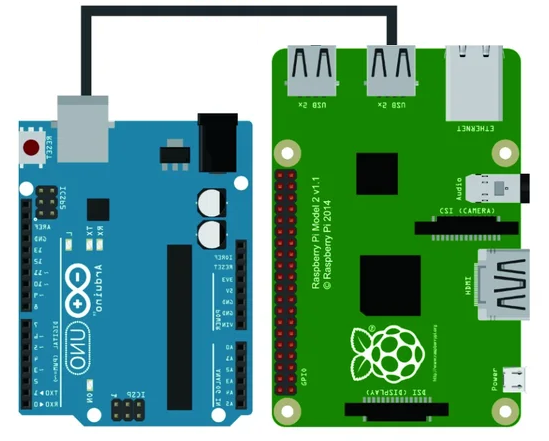
\includegraphics[scale=0.5]{Pictures/chapter08/usb.png}
  \caption{\small De \textit{Raspberry Pi} gekoppeld aan de \textit{Arduino} met een USB kabel.} 
\label{fig:usb} % Unique label used for referencing the figure in-text
%\addcontentsline{toc}{figure}{Figure \ref{fig:webserver}} % Uncomment to add the figure to the table of contents
\end{figure}

\begin{exercise}
  Sluit de \textit{Arduino} via USB aan op de \textit{Raspberry Pi}.
\end{exercise}
Onder Windows is de seriële poort, zoals je weet, te vinden als COM\textit{X}, waarbij \textit{X} een letter is (\textit{COM1}, \textit{COM5}, etc.). Omdat er op onze \textit{Raspberry Pi} een Linuxvariant (Raspberry Pi OS) draait, is het verstandig om even stil te staan bij hoe de seriële poort daar werkt.\newline

\newpage 

\subsection{Seriële poort in Linux}
Linux zit nogal anders in elkaar dan Windows. De menubalk die ineens bovenin zit, is het eerste wat in het oog schiet, maar dat is slechts het topje van de ijsberg. Wellicht heb je wel eens een file-explorer gestart, en dan zag het volgende: 
\begin{figure}[h!]
\centering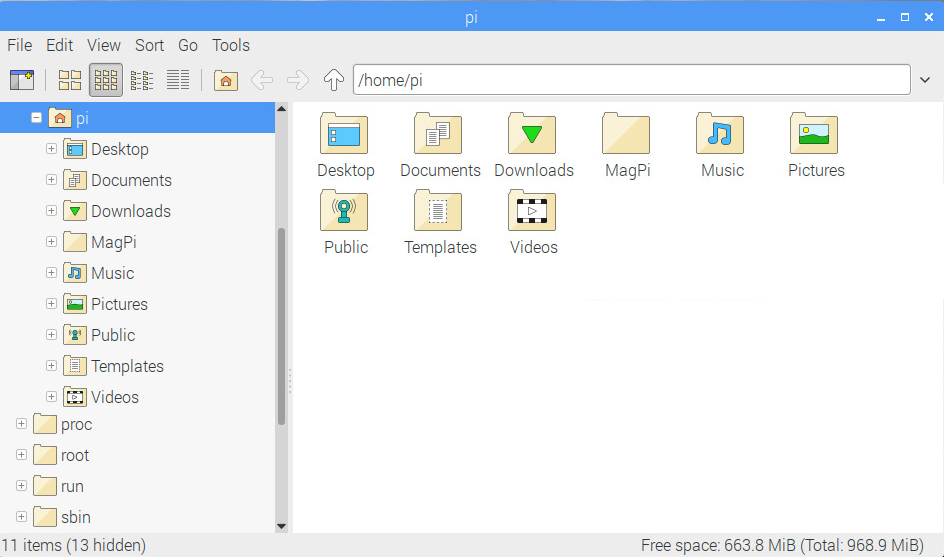
\includegraphics[scale=0.35]{Pictures/chapter08/home_folder.png}
  \caption{\small De home folder map met de bekende folders} 
\label{fig:home_folder} % Unique label used for referencing the figure in-text
%\addcontentsline{toc}{figure}{Figure \ref{fig:webserver}} % Uncomment to add the figure to the table of contents
\end{figure}

Dat komt waarschijnlijk redelijk bekend voor, de \textit{home} folder (voor de gebruiker \textit{pi}) lijkt nog redelijk op de folder \textit{Mijn Documenten} op Windows. Maar ga nu eens twee mapjes hoger. Je kom nu uit bij de zogeheten \textit{root-folder}, aangegeven met: '\textit{/}'. Deze is vergelijkbaar met de \textit{C:} schijf onder Windows. 
Waarschijnlijk vraag je je af wat dit allemaal voor vreemde folder zijn, en waar zit dan bijv. Linux geïnstalleerd er is namelijk geen '\textit{/linux}'-folder (zoals er onder windows wel een '\textit{C:\textbackslash Windows}'-folder is). Tja, dat is dus compleet anders hier. We gaan er niet te diep op in (want dat is een vak an sich), maar een beetje kennis ervan is wel handig als je hardware wil aansturen/uitlezen zoals de seriële poort.\newline

Onder Linux is 'alles een bestand'. Dus niet alleen je standaard tekst-bestanden, plaatjes, video's etc. maar alles. Dus bijv. alle programma's die je draait zijn te vinden onder de '\textit{/proc}'-folder (het tooltje \textit{top} en \textit{htop} halen bijv. hier al hun informatie weg). Informatie over de computer zelf (zoals het aanwezige geheugen en de CPU) kun je vinden in \textit{/sys}. En alle aangesloten hardware zijn te vinden onder \textit{/dev} (van devices). 

Bijv. je harde schijf zit hier (in het geval van de Pi, als \textit{/dev/mmcblk0}). Heb je een muis aangesloten? Dan is die te vinden hier als \textit{/dev/input/mouse0}. De aangesloten \textit{Arduino} is hier ook te vinden. De vraag is alleen welk bestand moet ik hiervoor hebben? \newline

Het handige daarvoor is om de \textit{Arduino} even los te koppelen en een terminal te openen op de \textit{Pi}. Typ nu het volgende in:
\begin{lstlisting}[language=bash]
ls /dev/tty*
\end{lstlisting}
Dit geeft een (flinke) lijst met apparaten. Sluit nu de \textit{Arduino} weer aan en voer de bovenstaande regel opnieuw uit. Het apparaat wat er nu bij gekomen is, is de \textit{Arduino}. Onthou deze.

\begin{remark}
  De \textit{Arduino} zal waarschijnlijk zitten op \textit{/dev/ttyUSB0} of \textit{/dev/ttyACM0}.
\end{remark}

\newpage 

% \subsubsection{Arduino code: Schrijven naar seriële poort}
Om de seriële poort uit te lezen zijn is het natuurlijk wel handig dat de \textit{Arduino} daar iets mee doet. We maken even snel een klein programmaatje op de Arduino die precies dat doet en laden dat erop:
\begin{lstlisting}[language=Arduino]
void setup() 
{
  Serial.begin(9600);
}

void loop() 
{
  Serial.println("Hallo vanaf Arduino!");
  delay(1000); // Wacht een seconde.
}
\end{lstlisting}
\begin{exercise}
  Laad het bovenstaande programma op je \textit{Arduino}. Je kunt 'm ook gewoon programmeren op de \textit{Pi} door daar de Arduino-IDE te gebruiken. Is hij toch nog niet geïnstalleerd? Dan:
  \begin{lstlisting}[language=bash]
  sudo apt install arduino
  \end{lstlisting}
\end{exercise}

\subsection{PySerial}

\begin{figure}[h!]
\centering
\includegraphics[scale=0.75]{Pictures/chapter08/pyserial.png}
\label{fig:pyserial} % Unique label used for referencing the figure in-text
%\addcontentsline{toc}{figure}{Figure \ref{fig:webserver}} % Uncomment to add the figure to the table of contents
\end{figure}

Tijd om te kijken of we de data die nu gestuurd wordt door de \textit{Arduino} kunnen lezen met de \textit{Pi} via \textit{Python}. Dit gaan we doen met een handige package genaamd \textit{PySerial}. 

\begin{remark}
  Als het goed is, is deze package standaard geïnstalleerd op de \textit{Pi}, zoniet (of als je 'm ook graag op je pc hebben) dan even onderstaande uitvoeren in een terminal:
  \begin{lstlisting}[language=bash]
    python3 -m pip install pyserial
  \end{lstlisting}
\end{remark}

Onderstaande stuk code is alles wat we hiervoor nodig hebben:
\inputpython{code/chapter08/arduino_serial.py}

We maken hierin een object genaamd \pyth{ser} aan, van het type \pyth{serial.Serial}. Dit object handeld alle communicatie af met de daadwerkelijke seriële poort. We moeten 'm alleen even vertellen met welke poort en met welke snelheid we willen praten.
Voordat dat we iets met de poort doen moeten we even wachten. \newline 
Door een wellicht wat onhandige ontwerpkeuze start de \textit{Arduino} opnieuw op als je de seriële poort opent. Hier is weinig aan te doen, als je hier niet wacht kan het zijn dat je een aantal berichten mis loopt, doordat de \textit{Arduino} nog aan het opstarten is terwijl jij al berichten verwacht. Daarna lezen we de poort $10$ keer uit en schrijven wat we terugkrijgen naar het scherm. Hetgeen wat we uitlezen is nog geen \pyth{str}, maar \pyth{bytes}, vandaar dat we de gelezen data nog even moeten omzetten. \newline

Het keyword \pyth{with} is hier nieuw. We kunnen het programma ook schrijven zonder:
\inputpython{code/chapter08/arduino_serial2.py}
Maar in dat geval moeten we als we klaar zijn met de poort, de functie \pyth{close()} aanroepen zodat de poort netjes wordt afgesloten. Met \pyth{with} gebeurt dit automatisch als het programma ermee klaar is. Het is aan te bevelen om het via \pyth{with} te doen. \newline

Als we deze code uitvoeren zullen we $10$ keer worden begroet door onze \textit{Arduino}, sympathiek!
\begin{python}
0: Hallo vanaf Arduino!
1: Hallo vanaf Arduino!
2: Hallo vanaf Arduino!
3: Hallo vanaf Arduino!
4: Hallo vanaf Arduino!
5: Hallo vanaf Arduino!
6: Hallo vanaf Arduino!
7: Hallo vanaf Arduino!
8: Hallo vanaf Arduino!
9: Hallo vanaf Arduino!
\end{python}

% \subsubsection{Arduino code: Lezen seriële poort}

Nu het uitlezen van data vanaf de \textit{Arduino} is gelukt, gaan we ons inleren hoe we het de communicatie de andere kant op kunnen opzetten. Hiervoor zijn we een Arduino programma nodig die data op de seriële poort inleest, en hier iets mee doet. In het volgende voorbeeld checkt ons programma of er een $1$ of een $0$ binnen komt, en zet op basis daarvan een Led (aangesloten op pin $d13$) aan of uit. 

\newpage 

\begin{lstlisting}[language=Arduino]
const int led_pin = 13;             // Led, aangesloten op d13

void setup() 
{
  Serial.begin(9600);
  pinMode(led_pin, OUTPUT);
}

void loop() 
{
  // Als er data is:
  if(Serial.available() > 0)
  {
    // Lees deze in:
    char data = Serial.read();
    if(data == '1')
    {
      digitalWrite(led_pin, HIGH);  // Doe led aan bij een '1'
    }
    else if(data == '0')
    {
      digitalWrite(led_pin, LOW);   // Doe led uit bij een '0'
    }
  }
}
\end{lstlisting}

Op de \textit{Pi} draaien we de volgende code, die eerst het character '$1$' stuurt en een seconde later het character '$0$':
\inputpython{code/chapter08/arduino_serial_write.py}
An sich is deze code redelijk recht-toe-recht-aan. Maar een belangrijk detail moet je zeker niet over het hoofd zien, op regel $7$ en $13$ sturen we de $1$ en $0$. Maar dit is geen standaard \pyth{str}, maar \pyth{bytes}. Intern werkt \textit{PySerial} enkel met \pyth{bytes}. Dus je strings moet je even omzetten voor je ze verstuurd of ontvangt. Dit kan door er een \pyth{b} voor te zetten, of door de functie \pyth{encode()} aan te roepen op je string.\newline
De ontvangen data moet je dus ook even opmaken (omzetten van \pyth{bytes} naar \pyth{str} via \pyth{decode()} en newline verwijderen met \pyth{strip()}). Dit kan direct bij het lezen (regel $14$), maar ook gerust bij het printen (regel $8$). Van de \textit{Arduino} krijgen we de volgende info terug:
\begin{python}
Ontvangen: Led on!
Ontvangen: Led off!
\end{python}

\newpage

\subsubsection{OOP variant}
Wat nu als we onze eerder opgedane kennis van OOP toe gaan passen op onze \textit{Arduino} communicatie. Dan moeten we eerst weer de standaardvragen stellen. Welke eigenschappen/variabelen heeft onze \textit{Arduino}? En welke functionaliteit moet hij bezitten? \newline
De arduino moet kunnen communiceren met een seriële poort, dus daar is hij een \pyth{Serial}-object voor nodig (die weer een poortnaam, baudrate en een timeout moet weten en waar we dan weer de functies \pyth{write()}, \pyth{readline()} en \pyth{close()} van gebruiken). En de \textit{Arduino} heeft op dit moment enkel een functie nodig die data kan zenden en dan direct een antwoord afvangt en teruggeeft. Dat kan in 1 functie.
\begin{figure}[h!]
\centering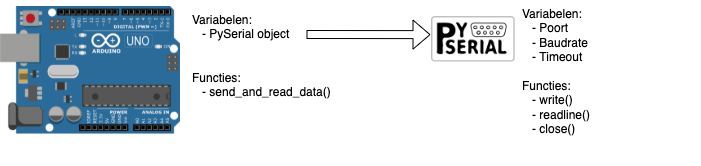
\includegraphics[scale=0.7]{Pictures/chapter08/arduino_oop.png}
\label{fig:arduino_oop} % Unique label used for referencing the figure in-text
%\addcontentsline{toc}{figure}{Figure \ref{fig:webserver}} % Uncomment to add the figure to the table of contents
\end{figure}

Als we dit in code uitwerken krijgen we de volgende klasse-definitie:
\inputpython{code/chapter08/arduino_serial_oop.py}

In de constructor (\pyth{__init__()}) van onze Arduino wordt de seriële poort (\pyth{serial}) geopend. Voor de poortname, snelheid (baudrate) en timeout, worden de waardes gebruikt die meegegeven worden in de constructor. Daarna wordt er $2$ gewacht, zodat de daadwerkelijke \textit{Arduino} even opnieuw kan opstarten. \newline

Op regel $12$ is de enige echte functie van onze Arduino klasse: \pyth{send_and_read_data()}, deze ontvangt een \pyth{str}, zet deze om naar \pyth{bytes} en verstuurd 'm over de seriële poort. Daarna wacht hij tot er data binnengekomen is met \pyth{readline()}, en deze data wordt weer opgemaakt (omgezet van \pyth{bytes} naar \pyth{str} en gestript) en teruggegeven. \newline

op regel $18$ is weer een nieuw iets te zien, een destructor (\pyth{__del__()}). Dit is de tegenhanger van de constructor. Waar de constructor wordt aangeroepen door \textit{Python} als je een nieuw object aanmaakt (\pyth{mijn_object =  Object(..)}), wordt de destructor aangeroepen als het object niet meer nodig is (bijv. als je programma klaar is, of wellicht heb je het object in een functie of if-statement aangemaakt en is die functie/statement afgerond). Dankzij deze destructor wordt de seriële poort altijd netjes afgesloten.
\begin{remark}
Je hoeft constructors en destructors dus alleen aan te maken. Deze worden intern en automatisch aangeroepen door \textit{Python}. 
\end{remark}

We hebben bovenstaande code opgeslagen in een bestand genaamt \pyth{arduino.py}. In een nieuw programma kunnen we deze dus weer importeren en gebruiken:
\begin{python}
from arduino import Arduino

# Maak nieuw object Arduino aan:
my_arduino = Arduino('/dev/ACM0', 9600)

# Stuur '1' en print ontvangen data:
data = my_arduino.send_and_read_data('1')
print(f'Ontvangen: {data}')

sleep(1)  # Even wachten

# Stuur '1' en print ontvangen data:
data = my_arduino.send_and_read_data('0')
print(f'Ontvangen: {data}')
# Hier wordt dus de Arduino-destructor aangeroepen.
\end{python}

Dit laat ook weer mooi een ander voordeel van OOP zien: abstractie. Alle technische details zitten verwerkt in onze \pyth{Arduino}-klasse, waardoor ons bovenstaande hoofdprogramma daardoor heel recht-toe-recht-aan blijft. 

\begin{exercise}
$\\$ Voeg aan de arduino-klasse $2$ functies toe: \pyth{on()} en \pyth{off()}, die lamp aan en uit laten gaan. \newline \newline
\textbf{TIP:} i.p.v. stukjes code kopiëren kun je ook \pyth{self.send_and_read_data()} gebruiken ;)
\end{exercise}

\newpage

\subsection{Ethernet}\index{Ethernet}
Naast een USB poort voor seriële communicatie hebben de \textit{Raspberry Pi} en de \textit{Arduino} een ethernetpoort (De \textit{Arduino} is hier uiteraard wel een schild voor nodig). 

\begin{figure}[h!]
\centering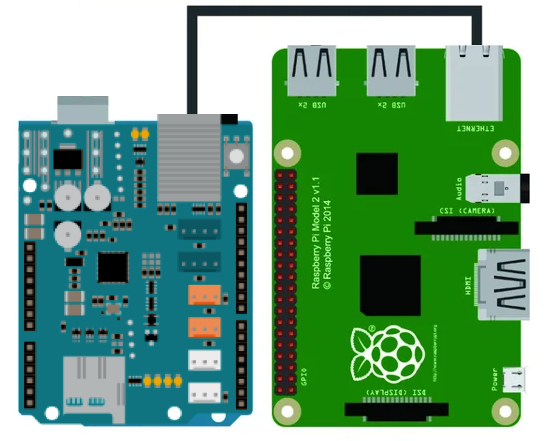
\includegraphics[scale=0.5]{Pictures/chapter08/ethernet.png}
\caption{\small De \textit{Raspberry Pi} gekoppeld aan de \textit{Arduino}+shield met een Ethernet kabel.}
\label{fig:ethernet} % Unique label used for referencing the figure in-text
%\addcontentsline{toc}{figure}{Figure \ref{fig:webserver}} % Uncomment to add the figure to the table of contents
\end{figure}

\begin{exercise}
Sluit de \textit{Arduino} met een Ethernetkabel aan op de \textit{Raspberry Pi}.
\end{exercise}

We gaan eerst even bekijken hoe je vanuit \textit{Python} via ethernet data kan versturen. Hiervoor zijn we uiteraard een stukje \textit{Arduino}-code voor nodig die die data kan ontvangen en bijv. naar de zijn seriële poort kan schrijven.

\lstinputlisting[language=Arduino]{code/chapter08/ethernetRec.ino}

\begin{exercise}
Laad het bovenstaande programma op je \textit{Arduino}. 
\end{exercise}

Voor het \textit{Python} programma maken we gebruik van de \pyth{socket} package, deze zit standaard in \textit{Python} (net als bijv. \pyth{math} en \pyth{time}) en kun/hoef je dus niet los installeren. Het jammere daaraan is dat het daarom geen kek logo heeft waarmee ik dit document kan opfleuren ;) \newline

Onderstaande programma gebruikt de \pyth{socket} package om een bericht te sturen:
\inputpython{code/chapter08/socket_send.py}

Het is inderdaad maar een kort programma. Maak een \pyth{socket}-object aan (regel $6$), zet de connectie op (regel $7$) op basis van het gegeven IP addres en poort en verstuur het bericht daarnaar toe. Omdat we weer een \pyth{with}-constructie gebruiken, hoeven we wederom niet de connectie zelf af te sluiten (\pyth{s.close()}), maar wordt dit dankzij \pyth{with} automatisch afgehandeld. \newline \newline

Nu dit werkt, rest natuurlijk de vraag hoe het de andere kant om werkt. In het geval dat de \textit{Arduino} iets stuurt en de \textit{Raspberry Pi} dit moet ontvangen. Ook hiervoor zijn we weer een simpel programmaatje nodig die zodra iemand connectie heeft gemaakt met de \textit{Arduino} begint met het sturen van data. In dit geval doet het programma dat eindeloos door, totdat de andere kant de connectie verbreekt. Als het goed is moet ook dit programma bekend voorkomen, gezien het een hele uitgeklede versie van de \textit{WebserverIO.ino} uit Hoofdstuk $1$.
\lstinputlisting[language=Arduino]{code/chapter08/ethernetSend.ino}

\newpage 

De bijbehorende code aan de \textit{Python} kant is iets minder triviaal als bij het ontvangen. 
\inputpython{code/chapter08/socket_recv.py}
We beginnen op dezelfde manier: we maken een \pyth{socket}-object aan (regel $6$), zet de connectie op (regel $8$) op basis van het gegeven IP addres en poort. We kunnen pas iets ontvangen nadat we als 'client' (de \textit{Arduino} is in dit geval de server), iets verstuurd hebben. Dus dat doen we op regel $11$, het maakt verder niet uit wat dit is. \newline

Daarna wordt er een beetje een truc toegepast. Normaal zou via dit soort verbindingen enkel een stroom aan data krijgen, en moet je van te voren aangeven hoeveel bytes je precies wil lezen. Maar in dit geval (op regel $14$) zeggen we dat we de binnengekomen data willen lezen alsof het een bestand is (\pyth{f}). Het voordeel daarvan is dat we die wel regel voor regel kunnen lezen. 
En dat is wat er daarna gebeurt, we lezen $10$ keer een regel uit ons (virtuele) bestand \pyth{f} en schrijven die naar het scherm. Waar we de vriendelijke begroeting van onze \textit{Arduino} zullen zien. 

\subsubsection{OOP variant}

\inputpython{code/chapter08/arduino_socket.py}

\begin{python}
from arduno_socket import ArduinoSocket

mijn_arduino = ArduinoSocket('192.168.1.3', 23)

for i in range(10):
    data = mijn_arduino.receive()
    print(f'{i}: {data}')

mijn_arduino.send('bla bla bla')

mijn_arduino.close()
\end{python}

% \subsection{MQTT?}\index{MQTT?}

% \begin{figure}[h!]
% \centering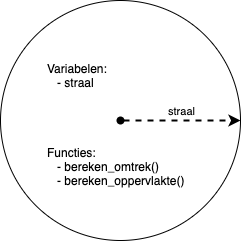
\includegraphics[scale=0.75]{Pictures/chapter07/cirkel.png}
% \caption{Ons cirkel-object heeft een straal, en kan (op basis daarvan) de omtrek en oppervlakte van zichzelf berekenen.}
% \label{fig:cirkel} % Unique label used for referencing the figure in-text
% %\addcontentsline{toc}{figure}{Figure \ref{fig:webserver}} % Uncomment to add the figure to the table of contents
% \end{figure}
%


% \newpage

% \section{Opdrachten}\index{Opdrachten}
% \begin{exercise}
% $\\$
% \end{exercise}

% \begin{exercise}
% $\\$
% \end{exercise}

% \begin{exercise}
% $\\$
% \end{exercise}

% \begin{exercise}
% $\\$
% \end{exercise}

% \begin{exercise}
% $\\$
% \end{exercise}

% \begin{exercise}
% $\\$
% \end{exercise}

% \begin{exercise}
% $\\$
% \end{exercise}

% \begin{exercise}
% $\\$
% \end{exercise}




%----------------------------------------------------------------------------------------
%	BIBLIOGRAPHY
%----------------------------------------------------------------------------------------

% \chapter*{Bronnen}
% \addcontentsline{toc}{chapter}{\textcolor{ocre}{Bibliography}} % Add a Bibliography heading to the table of contents

%------------------------------------------------

% \section*{Articles}
% \addcontentsline{toc}{section}{Articles}
% \printbibliography[heading=bibempty,type=article]
%
% %------------------------------------------------
%
% \section*{Books}
% \addcontentsline{toc}{section}{Books}
% \printbibliography[heading=bibempty,type=book]

%----------------------------------------------------------------------------------------
%	INDEX
%----------------------------------------------------------------------------------------

\cleardoublepage % Make sure the index starts on an odd (right side) page
\phantomsection
\setlength{\columnsep}{0.75cm} % Space between the 2 columns of the index
\addcontentsline{toc}{chapter}{\textcolor{ocre}{Index}} % Add an Index heading to the table of contents
\printindex % Output the index

%----------------------------------------------------------------------------------------

\end{document}
